\documentclass[12pt]{article}

\usepackage{amsmath}

\usepackage{graphicx}

\usepackage{hyperref}

\usepackage{graphicx}
\graphicspath{ {./images/} }

\usepackage{listings}
\usepackage{color}

\definecolor{dkgreen}{rgb}{0,0.6,0}
\definecolor{gray}{rgb}{0.5,0.5,0.5}
\definecolor{mauve}{rgb}{0.58,0,0.82}

\lstset{frame=tb,
  language=C,
  aboveskip=3mm,
  belowskip=3mm,
  showstringspaces=false,
  columns=flexible,
  basicstyle={\small\ttfamily},
  numbers=none,
  numberstyle=\tiny\color{gray},
  keywordstyle=\color{blue},
  commentstyle=\color{dkgreen},
  stringstyle=\color{mauve},
  breaklines=true,
  breakatwhitespace=true,
  tabsize=3
}

\usepackage[utf8]{inputenc}

\title{Operating System}
\author{Yuqiao Meng}
\date{2021–9–124}

\begin{document}

\maketitle

\newpage
\tableofcontents

\newpage

\section{Overview}

\subsection{What?}

What is an Operating System? What's its reponsibility?

\begin{itemize}
    \item A bunch of software and data residing somewhere in memory.
    \item The most privileged software in a computer. It  can do special things, like write to disk, talk over the network, control memory and CPU usage, etc
    \item Manages all system resources, including CPU, Memory, and I/O devices.
\end{itemize}

\subsection{Why?}
Why do we need an OS?
\begin{itemize}
    \item OS helps program to control hardwares.
    \item OS determines the way programs share resources.
    \item OS protects hardwares and programs from getting attacked.
    \item OS stores files persistently.
\end{itemize}
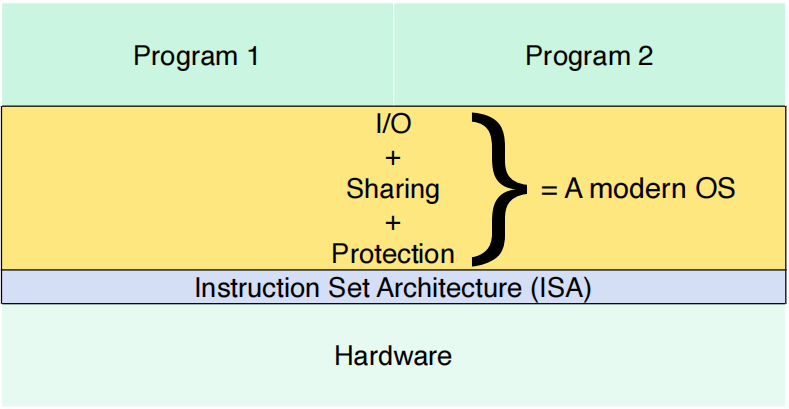
\includegraphics[width=1.0\textwidth]{WhyDoWeNeedOS.png}

\subsection{How}
\subsubsection{Virtualization}
\begin{itemize}
    \item Definition: OS takes a physical resource (such a sthe processor, or memory, or a disk) and transforms it into a more general, powerful, and easy-to-use virtual form of itself.
    \item Resource Virtualization \begin{itemize}
        \item Many(virtual)-to-one(physical): Virtual Machine
        \item One-to-many: Memory Virtualization
        \item Many-to-many: CPU Virtualization
    \end{itemize}
\end{itemize}
\subsubsection{How to invoke OS code?}
\begin{itemize}
    \item System calls: Function calls into the OS, that OS provides these calls to run programs, access memory and devices, and other related actions.
    \item Exceptions: CPU will raise an exception to the OS when the running program do something wrong
    \item Interrupts: Hardwares send interrupts to invoke OS
    \item Kernel Threads: Programs run in the kernel context, executing kernel level functions.
\end{itemize}
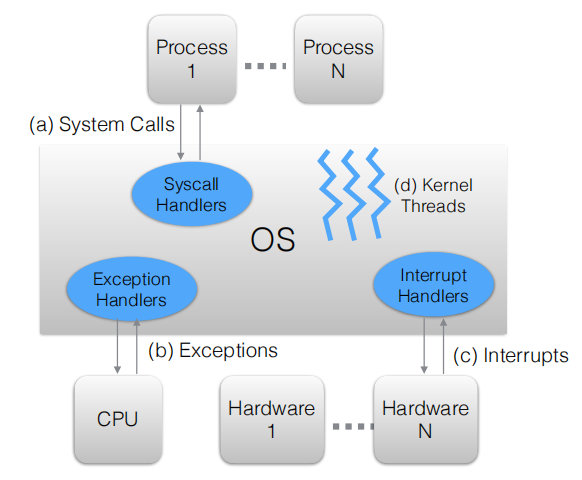
\includegraphics[width=0.8\textwidth]{FourWaysToInvokeOS.png}

\subsection{Interface}
\subsubsection{Explaination}
\begin{itemize}
    \item Instruction Set Architecture(ISA): the language CPU understand
    \item User ISA: ISA that any program can execute, it's accessible for all programs, doesn't need the service of operating system
    \item System ISA: ISA that only operating system is allowed to execute.
    \item Application Binary Interface(ABI): the combination of syscalls and User ISA(3, 7), it's the view of the world, seen by programs. It's the reason why a program complied on one OS cannot be just moved to another OS.
    \item Application Programmers' Interface(API): the combination of libraries and User ISA(2, 7), it's the tools programmer use to write codes.
\end{itemize}
\subsubsection{Interfaces in a Computer System}
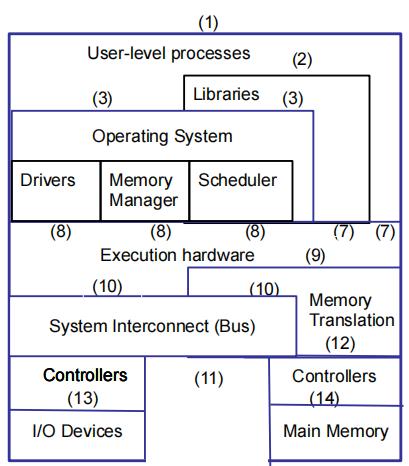
\includegraphics[width=0.6\textwidth]{InterfacesInComputerSystem.png}
\begin{itemize}
    \item User ISA: 7
    \item System ISA: 8
    \item Syscalls: 3
    \item Application Binary Interface: 3, 7
    \item Application Programmers' Interface: 2, 7
\end{itemize}

\subsection{History}
\begin{itemize}
    \item First Computer: Atanasoff–Berry computer, or ABC. ENIAC
    \item First OS: GM-NAA I/O, produced in 1956 by General Motors' Research division for its IBM 704.
    \item First language: Plankalkül, developed by Konrad Zuse for the Z3 between 1943 and 1945. Or FORTRAN
    \item First programmer: Ada Lovelace
\end{itemize}

\section{Processes}
\subsection{Process}
\subsubsection{What?}
What is a process?
\begin{itemize}
    \item A process is a program in execution. A program is a set of instructions somewhere (like the disk).
    \item Once created, a process continuously does the following: \begin{itemize}
        \item {\bfseries Fetches} an instruction from memory. 
        \item {\bfseries Decodes} it. i.e., figures out which instruction this is. 
        \item {\bfseries Executes} it. it does the thing that it is supposed to do, like add two numbers together, access memory, check a condition, jump to a function, and so forth.
    \end{itemize}
\end{itemize}

\subsubsection{Process versus Program}
How is a process different from a program?
\begin{itemize}
    \item Program: A passive entity stored in the disk, has static code and static data.
    \item Process: Actively executing code and the associated static and dynamic data.
    \item Program is just one component of a process.
    \item There can be multiple process instances of the same program
\end{itemize}

\subsubsection{Constitution}
\begin{itemize}
    \item Memory space
    \item Procedure call stack
    \item Registers and counters
    \item Open files, connections
    \item And more.
\end{itemize}

\subsubsection{Memory layout}
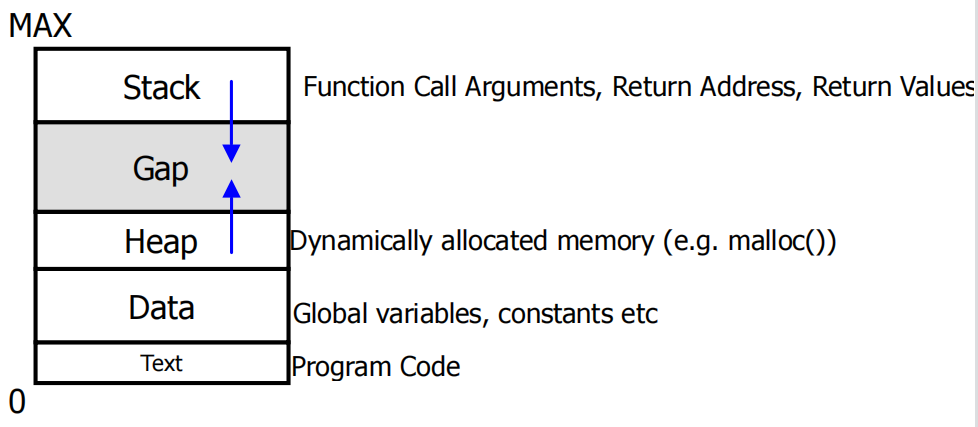
\includegraphics[width=1.0\textwidth]{ProcessMemoryLayout.png}
In this picture, Stack and Heap grow toward each other, that's because every process has a limited amount of space, thus let heap and stack grow toward each other from two direction can make the best use of space.

\subsection{System calls}
\begin{itemize}
    \item fork(): create new process. {\bfseries called once but return twice}. Usage: \begin{itemize}
        \item User runs a program at command line
        \item OS creates a process to provide a service: Check the directory /etc/init.d/ on Linux for scripts that start off different services at boot time.
        \item One process starts another process: For example in servers
    \end{itemize}
    \item exec(): execute a file. {\bfseries No return if Success. Replaces the process’ memory with a new program image. All I/O descriptors open before exec stay open after exec}.
    \item wait()/waitpid(): wait for child process.
    \item exit(): terminate a process
\end{itemize}

\subsection{Lifecycle}
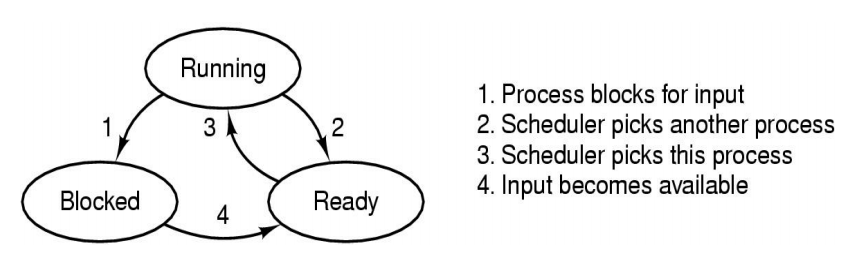
\includegraphics[width=1.0\textwidth]{ProcessLifecycle.png}
\begin{itemize}
    \item Ready (runnable; temporarily stopped to let another process run)\begin{itemize}
        \item Process is ready to execute, but not yet executing 
        \item Its waiting in the scheduling queue for the CPU scheduler to pick it up. 
    \end{itemize}
    \item Running:  (actually using the CPU at that instant) 
    \item Blocked (unable to run until some external event happens).\begin{itemize}
        \item Process is waiting (sleeping) for some event to occur. 
        \item Once the event occurs, process will be woken up, and placed on the scheduling queue
    \end{itemize}
\end{itemize}

\begin{enumerate}
    \item Running {$\to$} Blocked: Occurs when the operating system discovers that a process cannot continue right now.
    \item Running {$\to$} Ready: Occurs when the scheduler decides that the running process has run long enough and it is time to let another process have some CPU time.
    \item Ready {$\to$} Running: Occurs when all the other processes have had their fair share and it is time for the first process to get the CPU to run again.
    \item Blocked {$\to$} Ready: Occurs when the external event for which a process was waiting (such as the arrival of some input) happens
\end{enumerate}


\subsection{Special Process}
\begin{itemize}
    \item Orphan process \begin{itemize}
        \item When a parent process dies, child process becomes an orphan process
        \item The init process (pid = 1) becomes the parent of the orphan processes
    \end{itemize}
    \item Zombie process \begin{itemize}
        \item When a child dies, a SIGCHLD signal is sent to the OS, If parent doesn’t wait()on the child, and child exit()s, it becomes a zombie.
        \item Zombies hang around till parent calls wait() or waitpid().
        \item Zombies take up no system resources, it's just a integer status kept in the OS.
        \item Ways to prevent a child process from becoming a zombie: \begin{itemize}
            \item Parent call wait()/waitpid() before child process exit()
            \item Child parent sleep() before exit() until parent process give it a message.
            \item Set act.sa\_flags is SA\_NOCLDWAIT
        \end{itemize}
    \end{itemize}
\end{itemize}

\subsection{Cold-start Penalty}
\subsection{Context Switch}

\section{Inter-Process Communication}
\subsection{Overview}
Inter-Process Communication mechanisms
\begin{itemize}
    \item Pipe: A directional communication mechanism
    \item Signals: Event notification from one process to another
    \item Shared momery: Common piece of read/write memory, needs authorization for access
    \item Parent-child: Command-line arguments, including waitpid(), wait(), exit()
    \item Reading/modifying common files
    \item Semaphores: Locking and event signaling mechanism between processes
    \item Sockets: Not just across the network, but also between processes
\end{itemize}

\subsection{Pipe}
\subsubsection{Abstraction}
Write to one end, read from another.
\newline
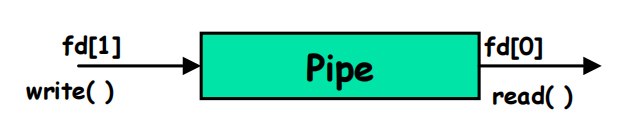
\includegraphics[width=0.8\textwidth]{PipeAbstraction.png}
\subsubsection{Parent-Child Communication Using Pipe}
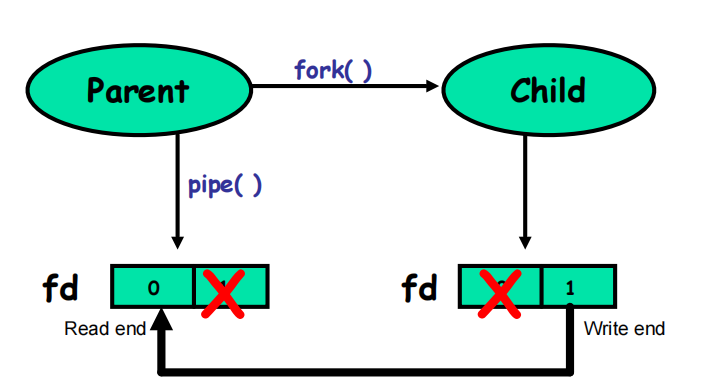
\includegraphics[width=0.8\textwidth]{ParentChildCommunicationUsingPipe.png}
\subsubsection{File-Descriptor Table}
\begin{itemize}
    \item Each process has a file-descriptor table
    \item One entry for each open file
    \item File includes regular file, stdin, stdout, pipes, etc.
\end{itemize}
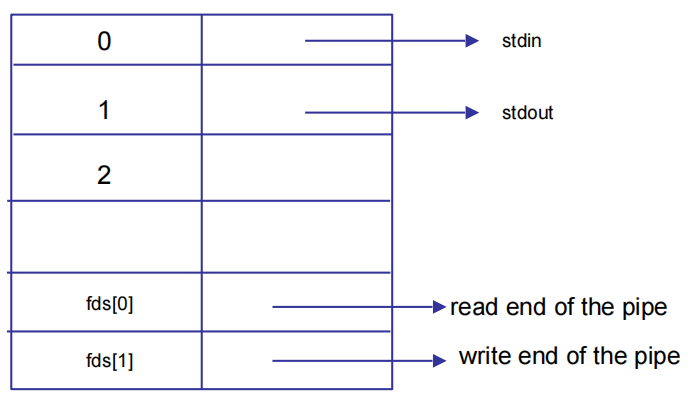
\includegraphics[width=0.8\textwidth]{FileDescriptorTable.png}
\subsubsection{Redirect Std to a File}
\begin{lstlisting}
#include <stdio.h>
#include <stdlib.h>
#include <errno.h>
#include <sys/types.h>
#include <unistd.h>

int main()
{
    int fds[2];
    char buf[30];
    pid_t pid1, pid2, pid;
    int status, i;

    /* create a pipe */
    if (pipe(fds) == -1) {
        perror("pipe");
        exit(1);
    }

    /* fork first child */
    if ( (pid1 = fork()) < 0) {
        perror("fork");
        exit(1);
    }

    if ( pid1 == 0 ) {
        close(1);  /* close normal stdout (fd = 1) */
        dup2(fds[1], 1);   /* make stdout same as fds[1] */
        close(fds[0]); /* we don't need the read end -- fds[0] */

        if( execlp("ps", "ps", "-elf", (char *) 0) < 0) {
            perror("Child");
            exit(0);
        }

	/* control never reaches here */
    } 

    /* fork second child */
    if ( (pid2 = fork()) < 0) {
	perror("fork");
	exit(1);
    }

    if ( pid2 == 0 ) {
        close(0);   /* close normal stdin (fd = 0)*/
        dup2(fds[0],0);   /* make stdin same as fds[0] */
        close(fds[1]); /* we don't need the write end -- fds[1]*/

        if( execlp("less", "less", (char *) 0) < 0) {
            perror("Child");
            exit(0);
        }

	/* control never reaches here */
    }

    /* parent doesn't need fds  - MUST close - WHY? */
    /* The reading side is supposed to learn that the writer has finished if it notices an EOF condition. This can only happen if all writing sides are closed.*/
    /* close its reading end (for not wasting FDs and for proper detection of dying reader)*/
    /* close its writing end (in order to be possible to detect the EOF condition).*/
    close(fds[0]); 
    close(fds[1]); 

    /* parent waits for children to complete */
    for( i=0; i<2; i++) {
	pid = wait(&status);
	printf("Parent: Child %d completed with status %d\n", pid, status);
    }

}

\end{lstlisting}
\subsubsection{Handling Chain of Filters Using Pipe}
\emph{command 1 $|$ command 2 $|$ … $|$ command N}
\begin{itemize}
    \item First command? \begin{itemize}
        \item Yes: continue
        \item No: redirect stdin to previous pipe
    \end{itemize}
    \item Last command? \begin{itemize}
        \item Yes: Output
        \item No: \begin{itemize}
            \item create next pipe (if needed)
            \item redirect stdout to next pipe
            \item fork a child for next level of recursion with one command less as input
        \end{itemize}
    \end{itemize}
    \item exec the command for the current level
\end{itemize}
\subsubsection{Byte-stream versus Message}
\begin{itemize}
    \item Byte-Stream abstraction: Pipe \begin{itemize}
        \item Can read and write at arbitrary byte boundaries
        \item Don't need to return explicit bytes of data. \emph{read(fds[0], buf, 6)} \begin{itemize}
            \item read() could reach end of input stream (EOF).
            \item Other endpoint may abruptly close the connection
            \item read() could return on a signal
        \end{itemize}
    \end{itemize}
    \item Message abstraction: Provides explicit message boundaries.
\end{itemize}
\subsubsection{Error Handling}
We must incorporate error handling with every I/O call (actually with any system call)
\begin{itemize}
    \item First check the return value of every read(…)/write(…) system call
    \item Then \begin{itemize}
        \item Wait to read/write more data
        \item Handle any error conditions
    \end{itemize}
\end{itemize}
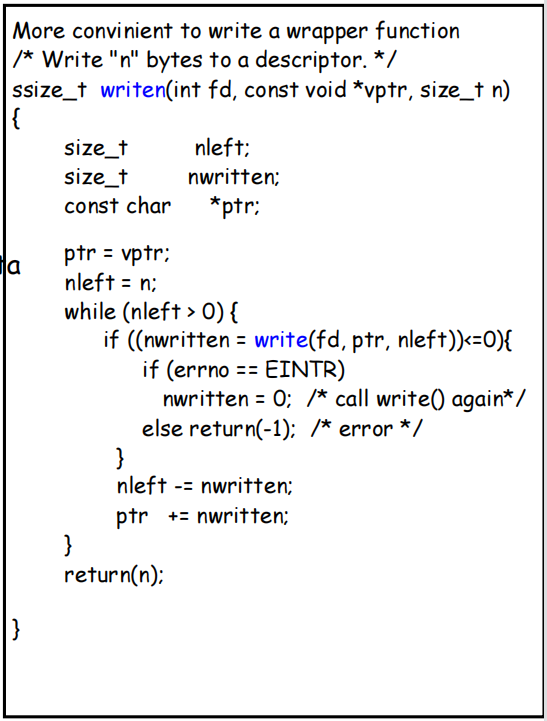
\includegraphics[width=0.8\textwidth]{PipeErrorHandling.png}

\subsection{Signals}
\subsubsection{Overview}
\begin{itemize}
    \item A notification to a process that an event has occurred, comes from OS or another process
    \item The type of event determined by the type of signal
\end{itemize}
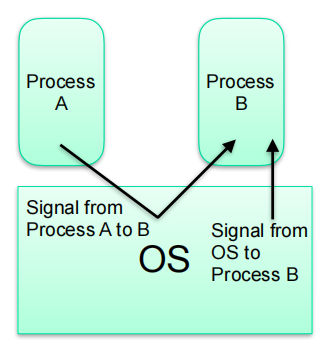
\includegraphics[width=0.6\textwidth]{SignalOverview.png}
\subsubsection{Handling Signals}
\begin{itemize}
    \item Signals can be {\bfseries caught} – i.e. an action (or handler) can be associated with them
    \item Actions can be customized using {\bfseries sigaction()}, which associates a signal handler with the signal
    \item {\bfseries Default} action for most signals is to \underline{terminate the process}. Except SIGCHLD and SIGURG are ignored by default
    \item Unwanted signals can be {\bfseries ignored}, except SIGKILL or SIGSTOP
\end{itemize}
\subsubsection{SIGCHLD}
\begin{itemize}
    \item Sent to parent when a child process terminates or stops
    \item If act.sa\_handler is SIG\_IGN, SIGCHLD will be ignored (default behavior)
    \item If act.sa\_flags is SA\_NOCLDSTOP, SIGCHLD won't be generated when children stop
    \item If act.sa\_flags is SA\_NOCLDWAIT, children of the calling process will not be transformed into zombies when they terminate
    \item These need to be set in sigaction() before parent calls fork()
\end{itemize}
Usage: handling child's exit without blocking on wait()
\begin{itemize}
    \item Parent could install a signal handler for SIGCHLD
    \item Call wait(…)/waitpid(…)inside the signal handler \begin{lstlisting}
        // sigchild.c
        void handle_sigchld(int signo) {
            pid_t pid;
            int stat;
 
            pid = wait(&stat); //returns without blocking 
            printf("child process exits.");
        }
        \end{lstlisting}
\end{itemize}

\subsection{Shared Memory}
\subsubsection{Overview}
Common chunk of read/write memory among processes.
\newline
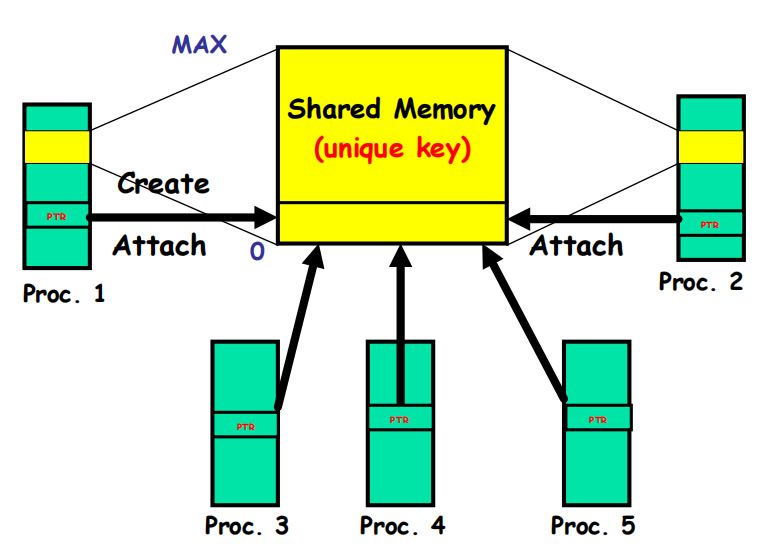
\includegraphics[width=0.8\textwidth]{SharedMemoryOverview.png}
\subsubsection{Creating}
\begin{lstlisting}
#include <stdio.h>
#include <stdlib.h>
#include <string.h>
#include <sys/types.h>
#include <sys/ipc.h>
#include <sys/shm.h>

#define SHM_SIZE 1024  /* make it a 1K shared memory segment */

int main(void)
{

       key_t key;
       int shmid;
       char *data;
       int mode;

       /* make the key: */
       /* The ftok() function uses the identity of the file named by the given pathname (which must refer to an existing, accessible file) and the least significant 8 bits of proj_id (which must be nonzero) to generate a key_t type System V IPC key, suitable for use with msgget(2), semget(2), or shmget(2). */
       /* The resulting value is the same for all pathnames that name the same file, when the same value of proj_id is used.  The value returned should be different when the (simultaneously existing) files or the project IDs differ.*/
       if ((key = ftok("test_shm", 'X')) < 0) {
            perror("ftok");
            exit(1);
       }

       /* create the shared memory segment: */
       /* shmget() returns the identifier of the System V shared memory segment associated with the value of the argument key.  It may be used either to obtain the identifier of a previously created shared memory segment (when shmflg is zero and key does not have the value IPC_PRIVATE), or to create a new set.*/
       /* A new shared memory segment, with size equal to the value of size rounded up to a multiple of PAGE_SIZE, is created if key has the value IPC_PRIVATE or key isn't IPC_PRIVATE, no shared memory segment corresponding to key exists, and IPC_CREAT is specified in shmflg.*/
       /* If shmflg specifies both IPC_CREAT and IPC_EXCL and a shared memory segment already exists for key, then shmget() fails with errno set to EEXIST.  (This is analogous to the effect of the combination O_CREAT | O_EXCL for open(2).) */
       /* 0644 means permissions of owner, group and user */
       if ((shmid = shmget(key, SHM_SIZE, 0644 | IPC_CREAT | IPC_EXCL )) < 0) {
            perror("shmget");
            exit(1);
       }

       return(0);
}
\end{lstlisting}
\subsubsection{Attach and Detach}
\begin{lstlisting}
#include <stdio.h>
#include <stdlib.h>
#include <string.h>
#include <sys/types.h>
#include <sys/ipc.h>
#include <sys/shm.h>

#define SHM_SIZE 1024  /* make it a 1K shared memory segment */

int main(int argc, char *argv[])
{

       key_t key;
       int shmid;
       char *data;
       int mode;


       /* make the key: */
       if ((key = ftok("test_shm", 'X')) == -1) {
            perror("ftok");
            exit(1);
       }


       /* connect to the segment. */
	   /* There's no IPC_CREATE. Because if there was one this function would create a new shared memory.*/
       if ((shmid = shmget(key, SHM_SIZE, 0644)) == -1) {
            perror("shmget");
            exit(1);
       }


	    /* attach to the segment to get a pointer to it: */
        /* The shmat() function attaches the shared memory segment associated with the shared memory identifier specified by shmid to the address space of the calling process.*/
        data = shmat(shmid, (void *)0, 0);
        if (data == (char *)(-1)) {
            perror("shmat");
            exit(1);
        }


        /* read or modify the segment, based on the command line: */
        if (argc == 2) {
            printf("writing to segment: \"%s\"\n", argv[1]);
            strncpy(data, argv[1], SHM_SIZE);
        } else
            printf("segment contains: \"%s\"\n", data);


        /* detach from the segment: */
        if (shmdt(data) == -1) {
            perror("shmdt");
            exit(1);
        }

       return(0);
}
\end{lstlisting}
\subsubsection{Deleting}
\begin{lstlisting}
#include <stdio.h>
#include <stdlib.h>
#include <string.h>
#include <sys/types.h>
#include <sys/ipc.h>
#include <sys/shm.h>

#define SHM_SIZE 1024  /* make it a 1K shared memory segment */

int main(void)
{
       key_t key;
       int shmid;
       char *data;
       int mode;

       /* make the key: */
       if ((key = ftok("test_shm", 'X')) == -1) {
            perror("ftok");
            exit(1);
       }

       /* connect to memory segment: */
       if ((shmid = shmget(key, SHM_SIZE, 0644)) == -1) {
            perror("shmget");
            exit(1);
       }

       /* delete he segment */
       /* IPC_RMID: Remove the shared memory identifier specified by shmid from the system and destroy the shared memory segment and shmid_ds data structure associated with it. IPC_RMID can only be executed by a process that has an effective user ID equal to either that of a process with appropriate privileges or to the value of shm_perm.cuid or shm_perm.uid in the shmid_ds data structure associated with shmid.*/
       if( shmctl(shmid, IPC_RMID, NULL) == -1) {
            perror("shmctl");
            exit(1);
       }

       return(0);
}
\end{lstlisting}
\subsubsection{Command}
\begin{itemize}
    \item ipcs: Lists all IPC objects owned by the user 
    \item ipcrm: Removes specific IPC object
\end{itemize}

\section{Threads}
\subsection{Problem}
Want to do multiple tasks Concurrently
\begin{itemize}
    \item Start two processes \begin{itemize}
        \item fork() is expensive
        \item cold-start penalty
    \end{itemize}
\end{itemize}
Processes may need to talk to each other
\begin{itemize}
    \item Two different address spaces, so we need to use IPC \begin{itemize}
        \item kernel transitions are expensive
        \item May need to copy data from a user to kernel to another user
        \item Inter-process Shared memory is a pain to set up
    \end{itemize}
\end{itemize}
\subsection{Solution}
\subsubsection{Event-driven programming}
\begin{itemize}
    \item Make one process do all the tasks 
    \item Busy loop polls for events and executes tasks for each event 
    \item No IPC needed 
    \item {\bfseries Length of the busy loop} determines response latency 
    \item Stateful event responses complicate the code
\end{itemize}
\begin{lstlisting}
while(1) 
{ 
    Check pending events; 
    if (event 1) do task 1; 
    if (event 2) do task 2; 
    // ...
    if (event N) do task N; 
}
\end{lstlisting}
\subsubsection{Threads}
Multiple threads of execution per process
\subsection{Threads}
Shared Resource
\begin{itemize}
    \item virtual address space(code, heap and static data)
    \item Open descriptors (files, sockets etc)
    \item Signals and Signal handlers
\end{itemize}
Non-Shared resources
\begin{itemize}
    \item Program counter
    \item Stack, stack pointer
    \item Registers
    \item Thread ID 
    \item Errno 
    \item Priority
\end{itemize}
\subsubsection{Address space layout}
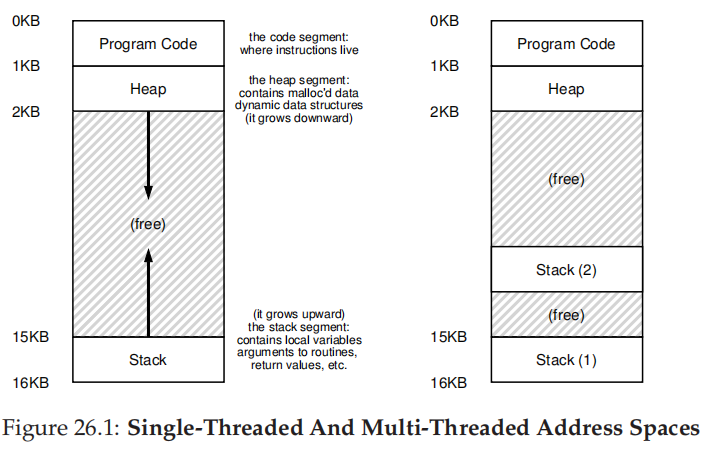
\includegraphics[width=\textwidth]{ThreadAddressSpace.png}
\subsubsection{Advantages}
\begin{itemize}
    \item Lower inter-thread context switching overhead than processes 
    \item No Inter-process communication \begin{itemize}
        \item Zero data transfer cost between threads 
        \item Only need inter-thread synchronization 
    \end{itemize}
    \item Threads can be pre-empted at any point \begin{itemize}
        \item Long-running threads are OK 
        \item As opposed to event-driven tasks that must be short. 
    \end{itemize}
    \item Threads can exploit parallelism, but it depends…more later 
    \item Threads could block without blocking other threads, but it depends … more later 
\end{itemize}
\subsubsection{Disadvantages}
\begin{itemize}
    \item Shared State! \begin{itemize}
        \item Global variables are shared between threads. 
        \item Accidental data changes can cause errors. 
    \end{itemize}
    \item Threads and signals don’t mix well \begin{itemize}
        \item Common signal handler for all threads in a process 
        \item Which thread to signal? Everybody! 
        \item Royal pain to program correctly. 
    \end{itemize}
    \item Lack of robustness. Crash in one thread will crash the entire process. 
    \item Some library functions may not be thread-safe \begin{itemize}
        \item Library Functions that return pointers to static internal memory. E.g. gethostbyname() 
        \item Less of a problem these days.
    \end{itemize}
\end{itemize}
\subsubsection{Types of Threads}
User-level threads
\begin{itemize}
    \item User-level libraries provide multiple threads,
    \item OS kernel does not recognize user-level threads
    \item Threads execute when the process is scheduled
\end{itemize}
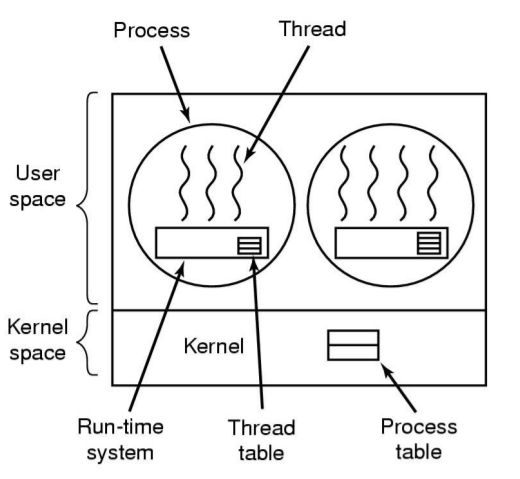
\includegraphics[width=0.6\textwidth]{UserLevelThreads.png}
\newline
Kernel-level threads
\begin{itemize}
    \item OS kernel provides multiple threads per process
    \item Each thread is scheduled independently by the kernel’s CPU scheduler
\end{itemize}
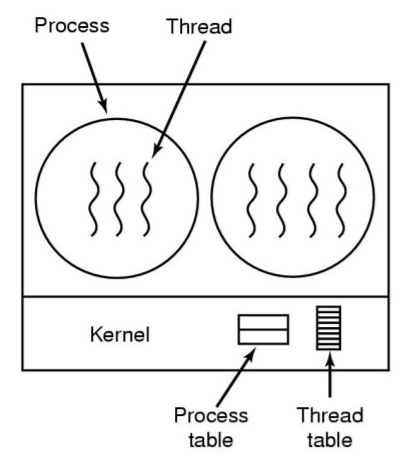
\includegraphics[width=0.6\textwidth]{KernelLevelThreads.png}
\newline
Hybrid Implementations
\newline
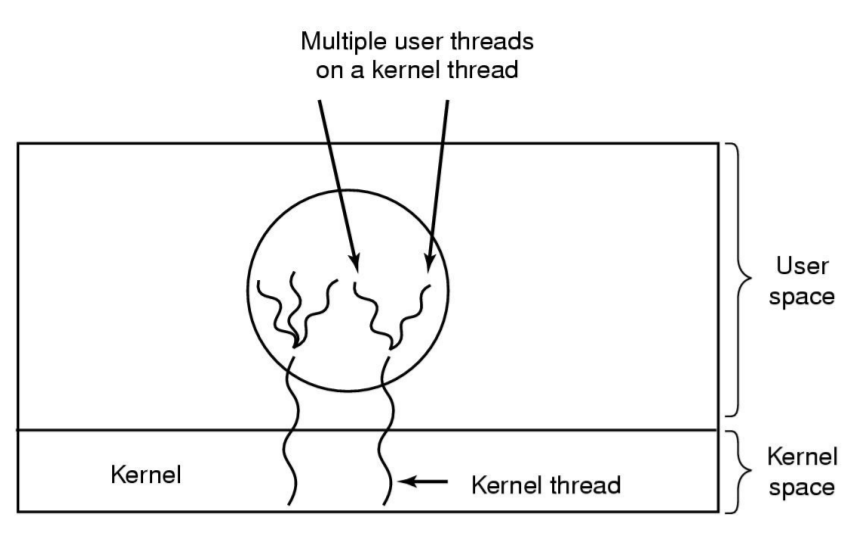
\includegraphics[width=0.6\textwidth]{MultiplexingThreads.png}
\newline
Multiplexing user-level threads within each kernel- level threads
\subsubsection{Scheduling}
Local Thread Scheduling
\newline
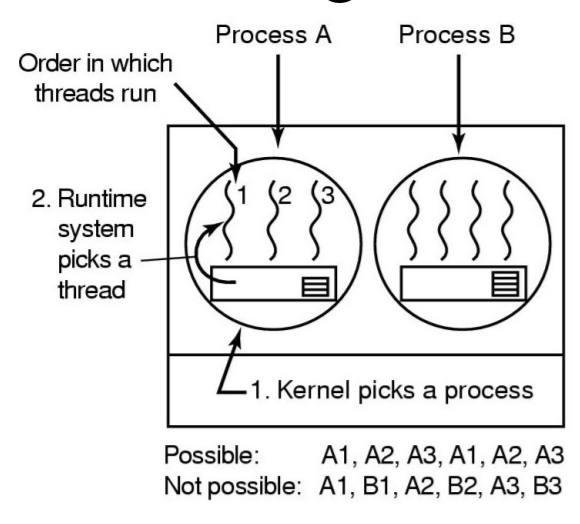
\includegraphics[width=0.6\textwidth]{LocalThreadScheduling.png}
\begin{itemize}
    \item Next thread is picked from among the threads belonging to the \emph{current process}
    \item Each process gets a timeslice from kernel
    \item Then the timeslice is \emph{divided up} among the threads within the current process 
    \item Local scheduling can be implemented with either Kernel-level Threads or user-level threads
    \item Scheduling decision requires only \emph{local knowledge} of threads within the current process.
\end{itemize}
Global Thread Scheduling
\newline
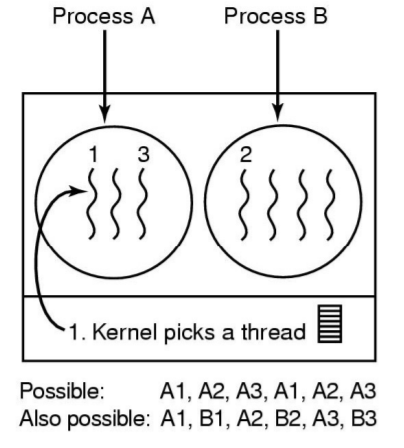
\includegraphics[width=0.6\textwidth]{GlobalThreadScheduling.png}
\begin{itemize}
    \item Next thread to be scheduled is picked up from \emph{ANY} process in the system. 
    \item Timeslice is allocated at the granularity of threads 
    \item Global scheduling can be implemented only with kernel-level threads: for Picking the next thread requires global knowledge of threads in all processes.
\end{itemize}
\subsubsection{Thread Creation and Termination}
\begin{itemize}
    \item Creation \begin{lstlisting}
        int pthread_create( pthread_t * thread, pthread_attr_t * attr,
        void * (*start_routine)(void *), void * arg);
    \end{lstlisting}
    \item Two ways to perform thread termination \begin{itemize}
        \item Return from initial function \begin{lstlisting}
            void pthread_exit(void * status)
        \end{lstlisting}
    \end{itemize}
    \item Waiting for child thread in parent \begin{itemize}
        \begin{lstlisting}
            pthread_join()
        \end{lstlisting}
        \item equivalent to waitpid
    \end{itemize}
\end{itemize}
\subsubsection{Code}
Example
\begin{lstlisting}
    // shared counter to be incremented by each thread
    int counter = 0;
    main()
    {
        pthread_t tid[N];
        for (i=0;i<N;i++) {
            /*Create a thread in thread_func routine*/
            Pthread_create(&tid[i], NULL, thread_func, NULL);
        }
        for(i=0;i<N;i++) {
            /* wait for child thread */
            Pthread_join(tid[i], NULL);
        }
        void *thread_func(void *arg)
        {
            /* unprotected code race condition */
            counter = counter + 1;
        }
        return NULL; // thread dies upon return
    }
\end{lstlisting}
\subsubsection{pthread Synchronization Operations}
\begin{lstlisting}
    // Mutex operation
    pthread_mutex_init()
    pthread_mutex_lock()
    pthread_mutex_unlock ()
    pthread_mutex_trylock ()

    // Condition variables
    pthread_cond_wait ()
    pthread_cond_signal ()
    pthread_cond_broadcast ()
    pthread_cond_timedwait ()
\end{lstlisting}

\section{Concurrency}
\subsection{Overview}
\begin{itemize}
    \item Sequential: one after another(two tasks executed on one CPU one after another)
    \item Concurrent: "juggling" many things within a time window(two tasks share a single CPU over time)
    \item Parallel: do many things simultaneously(two threads executing on two different CPUs simultaneously)
\end{itemize}
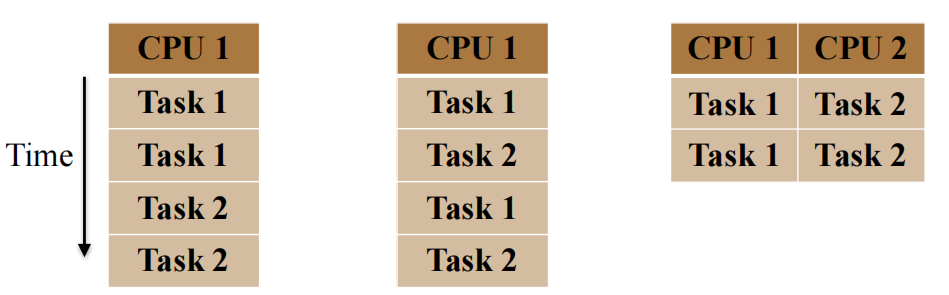
\includegraphics[width=0.8\textwidth]{ConcurrencyOverview.png}
\newline
Concurrent tasks must be either
\begin{itemize}
    \item execute independently
    \item synchronize the shared resource \begin{itemize}
        \item Shared memory
        \item Pipes
        \item Signals
    \end{itemize}
\end{itemize}
\subsection{Critical Section}
\begin{itemize}
    \item Definition: A section of code in a concurrent task that {\bfseries modifies or accesses} a resource shared with another task.
    \item Example: A piece of code that reads from or writes to a shared memory region
\end{itemize}
\subsection{Race Condition and Deadlocks}
\begin{itemize}
    \item Race Condition: Incorrect behavior of a program due to concurrent execution of critical sections by two or more threads
    \item Deadlocks: When two or more processes stop making progress {\bfseries indefinitely} because they are all waiting for each other to do something
\end{itemize}
\subsubsection{Mutual Exclusion}
Don’t allow two or more processes to execute their critical sections concurrently (on the same resource)
\newline
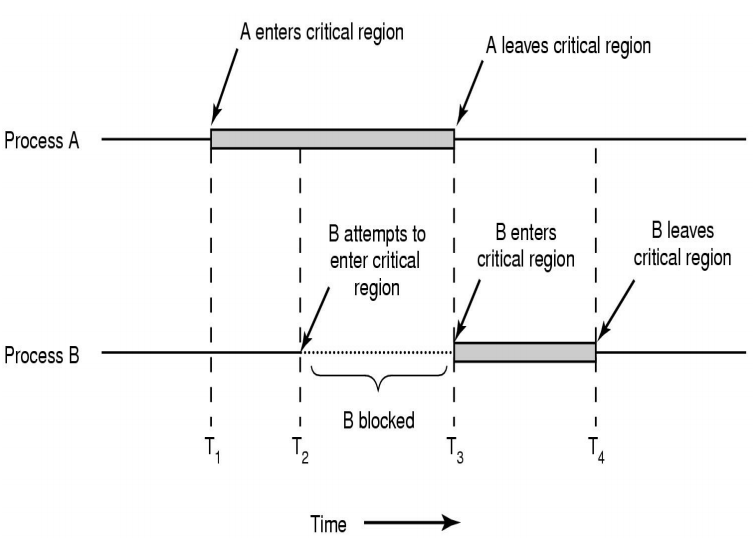
\includegraphics[width=0.8\textwidth]{MutualExclusionOverview.png}
\subsubsection{Conditions for correct mutual exclusion}
\begin{itemize}
    \item No two processes are simultaneously in the critical section 
    \item No assumptions are made about speeds or numbers of CPUs 
    \item No process must wait forever to enter its critical section. Waiting forever indicates a \emph{deadlock}
    \item No process running outside its critical region may block another process running in the critical section
\end{itemize}
The first two conditions are  enforced by the operating system’s implementation of locks, but the other two conditions have to be ensured by the programmer using the locks.
\subsubsection{Typs of Locks}
\begin{itemize}
    \item Blocking locks \begin{itemize}
        \item Give up CPU till lock becomes available \begin{lstlisting}
while(lock unavailable)
    yield CPU to others; // or block till lock available        
return success;
            \end{lstlisting}
        \item Usage: \begin{lstlisting}
Lock(resource); // Claim a shared resource
Execute Critical Section;//access or modify the shared resource
Unlock(resource); // unclaim shared resource
        \end{lstlisting}
        \item Advantage: Simple to use. Locking always succeeds…ultimately
        \item Disadvantage: Blocking duration may be indefinite \begin{itemize}
            \item Process is moved out of "Running" state to "Blocked" state, and return to running will cost much resource
            \item Delay in getting back to running state if lock becomes available soon after blocking
        \end{itemize}
    \end{itemize}
    \item Non-blocking locks \begin{itemize}
        \item Don’t block if lock is unavailable \begin{lstlisting}
if(lock unavailable)
    return failure;
else
    return success
        \end{lstlisting}
        \item Usage \begin{lstlisting}
if(TryLock(resource) == success)
    Execute Critical Section;
    Unlock(resource);
else
    Do something else; // plan B
        \end{lstlisting}
        \item Advantage: No unbounded blocking
        \item Disadvantage: Need a "plan B" to handle locking failure
    \end{itemize}
    \item Spin locks \begin{itemize}
        \item Don’t block. Instead, constantly poll the lock for availability \begin{lstlisting}
while (lock is unavailable) 
continue; // try again
return success;
        \end{lstlisting}
        \item Usage: Just like blocking locks \begin{lstlisting}
SpinLock(resource);
Execute Critical Section;
SpinUnlock(resource);
        \end{lstlisting}
        \item Advantage: Very efficient with short critical sections, if you expect a lock to be released quickly
        \item Disadvantage: \begin{itemize}
            \item Doesn’t yield the CPU and wastes CPU cycles, Bad if critical sections are long: P1 is in the ready queue, but P2 is doing spin with CPU until scheduler interrupts it and give CPU to P1
            \item Efficient only if machine has multiple CPUs
        \end{itemize}
    \end{itemize}
\end{itemize}
\subsubsection{Best practices for locking}
\begin{itemize}
    \item {\bfseries Associate locks with shared resources, NOT code.}
    \item {\bfseries Guard each shared resource by a separate lock.}
    \item {\bfseries OS cannot enforce these properties}
\end{itemize}
\subsubsection{Deadlock Solution}
Deadlock can only be prevented, once it happens, programmers can't solve it by killing the process or enforcing the process to give up the lock.
\newline
Right Solution: Lock Ordering
\begin{itemize}
    \item Sort the locks in a fixed order (say L1 followed by L2) 
    \item Always acquire subset of locks in the sorted order.
\end{itemize}
\subsubsection{Priority Inversion}
Conditions
\begin{itemize}
    \item static priority system
    \item synchronization between processes
\end{itemize}
Example
\begin{itemize}
    \item Definition: \begin{itemize}
        \item Ph – High priority 
        \item Pm – Medium priority 
        \item Pl – Low priority
    \end{itemize}
    \item Procedure \begin{itemize}
        \item Pl acquires a lock L 
        \item Pl starts executing critical section 
        \item Ph tries to acquire lock L and blocks 
        \item Pm becomes "ready" and preempts Pl from the CPU. 
        \item Pl might never exit critical section if Pm keeps preempting Pl
        \item So Ph might never enter critical section
    \end{itemize}
    \item Problem: A high priority process Ph is blocked waiting for a low priority process Pl, Pl cannot proceed because a medium priority process Pm is executing
    \item Solution: Priority Inheritance \begin{itemize}
        \item Temporarily increase the priority of Pl to HIGH PRIORITY 
        \item Pl will be scheduled and will exit critical section quickly 
        \item Then Ph can execute
    \end{itemize}
\end{itemize}
\subsubsection{Interrupts and Locks}
\begin{itemize}
    \item Interrupts invoke \emph{interrupt service routines (ISR)} in the kernel \begin{itemize}
        \item ISR must process the interrupt quickly and return: because there may be some other pending interrupts waiting to be delivered.
        \item So ISRs must \emph{never block or spin on a lock}.
    \end{itemize}
\end{itemize}
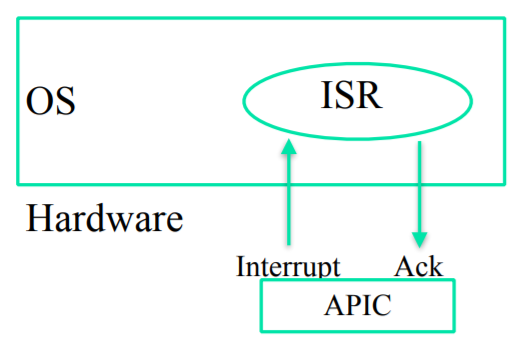
\includegraphics[width=0.6\textwidth]{InterruptServiceRoutine.png}
\subsubsection{Interrupts and Deadlocks — Problem}
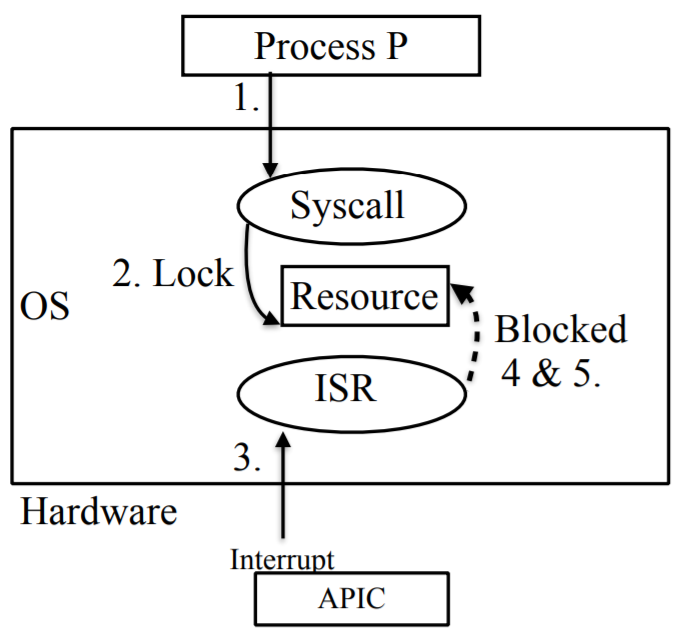
\includegraphics[width=0.6\textwidth]{InterruptAndDeadlock.png}
\begin{enumerate}
    \item P makes a syscall.
    \item Syscall acquires lock
    \item ISR preempts P* \emph{But P is still in the running state}
    \item ISR attempts to lock
    \item ISR blocks (since lock is taken)
    \item Deadlock!    
\end{enumerate}
\subsubsection{Interrupts and Deadlocks — Solutions}
\begin{enumerate}
    \item Don’t lock in ISR!: Defer any locking work to thread context (softirqs in Linux)
    \item If you must lock, use {$try lock()$} instead of lock() in ISR \begin{itemize}
        \item {$try lock()$} = if lock is available then get it, else return with error
        \item Write code to handle unavailable lock
    \end{itemize}
    \item Or disable interrupts in thread T before locking \begin{itemize}
        \item If ISR cannot run when lock is acquired by T, then there’s no deadlock.
        \item When ISR runs, it assumes that T doesn’t have the lock.
        \item But, disabling interrupts too long is also not a good idea.
    \end{itemize}
\end{enumerate}

\section{Semaphores, Condition Variables, Producer Consumer Problem}
\subsection{Semaphores}
\subsubsection{Definition}
Can be seen as a non-negative integer
\begin{itemize}
    \item Semaphore is a fundamental synchronization primitive used for \begin{itemize}
        \item Locking around critical regions 
        \item Inter-process synchronization
    \end{itemize}
    \item A semaphore "sem" is a special integer on which only two operations can be performed \begin{itemize}
        \item DOWN(sem)
        \item UP(sem)
    \end{itemize}
\end{itemize}
\subsubsection{DOWN(sem) Operation}
\begin{itemize}
    \item If (sem \textgreater \ 0) then \begin{itemize}
        \item Decrements sem by 1 
        \item The caller continues executing. 
        \item This is a {\bfseries successful} down operation.
    \end{itemize}
    \item If (sem == 0) then \begin{itemize}
        \item Block the caller 
        \item The caller blocks until another process calls an UP. 
        \item The blocked process wakes up and tries DOWN again. 
        \item If it succeeds, then it moves to {\bfseries ready} state 
        \item Otherwise it is blocked again till someone calls UP. 
        \item And so on
    \end{itemize}
\end{itemize}
\subsubsection{UP(sem) Operation}
\begin{itemize}
    \item This operation increments the semaphore sem by 1. 
    \item If the original value of the semaphore was 0, then UP operation wakes up {\bfseries all processes} that were sleeping on the DOWN(sem) operation. 
    \item All woken up processes compete to perform DOWN(sem) again. Only one of them succeeds and the rest are blocked again.
\end{itemize}
\subsubsection{Mutex}
A simply binary semaphore
\begin{itemize}
    \item Used as a LOCK around critical sections
    \item Locking a mutex means calling Down(mutex)
    \item Unlocking a semaphore means calling UP(mutex)
\end{itemize}
\subsection{Producer-Consumer Problem}
\subsubsection{Definition}
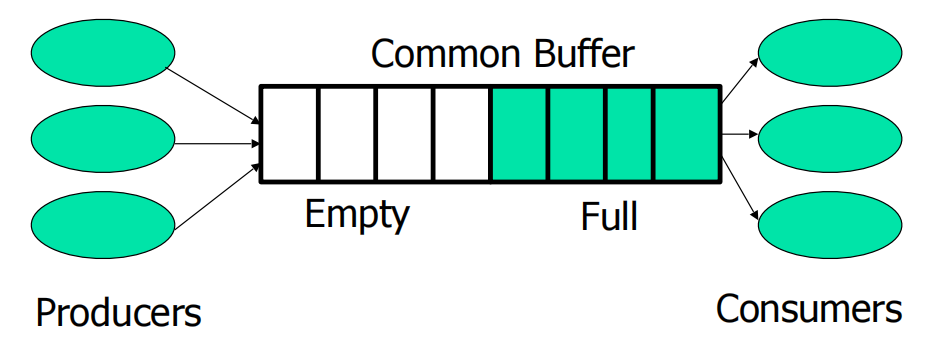
\includegraphics[width=0.8\textwidth]{Producer-ConsumerProblem.png}
\begin{itemize}
    \item Producers and consumers run in concurrent processes.
    \item Producers produce data and consumers consume data.
    \item Producer informs consumers when data is available
    \item Consumer informs producers when a buffer is empty.
    \item Three types of synchronization needed \begin{itemize}
        \item Locking the buffer to prevent concurrent modification
        \item Locking the buffer to prevent concurrent modification and getting
        \item Informing the other side that data/buffer is available
    \end{itemize}
\end{itemize}
\subsubsection{Solution}
\begin{lstlisting}
#define N 100
typedef int semaphore;
semaphore mutex = 1;
semaphore empty = N;
semaphore full = 0;

void producer(void){
    int item;
    while(true){
        item = produce_item();
        down(&empty);
        down(&mutex);
        insert_item(item);
        up(&mutex);
        up(&full);
    }
}

void consumer(void){
    int item;
    while(true){
        down(&full);
        down(&mutex);
        item = remove_item();
        up(&mutex);
        up(&empty);
        consume_item(item);
    }
}
\end{lstlisting}
\subsubsection{Using Semaphore}
\subsubsection{POSIX interface}
\begin{itemize}
    \item $sem\_open()$
    \item $sem\_init()$
    \item $sem\_wait(), sem_trywait()$
    \item $sem\_post()$
    \item $sem\_close()$
    \item $sem\_destroy()$
    \item $sem\_getvalue()$
    \item $sem\_unlink()$ -- Ends the connection to an open semaphore and causes the semaphore to be removed when the last process closes it.
\end{itemize}

\subsection{Monitors and Condition Variables}
\subsubsection{Definition}
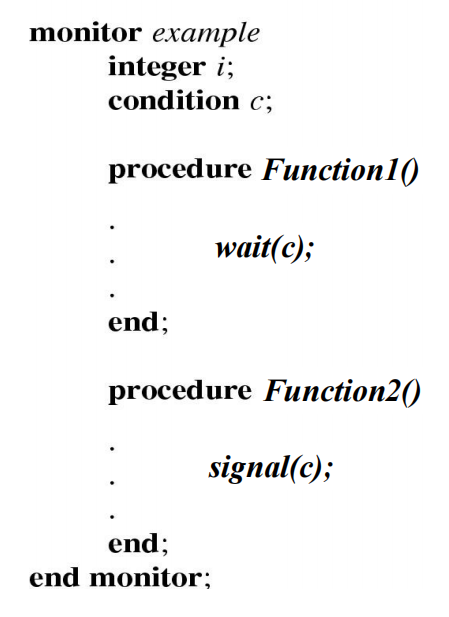
\includegraphics[width=0.6\textwidth]{Monitor.png}
\begin{itemize}
    \item Monitor is a collection of critical section procedures (functions): i.e. functions that operate on shared resources 
    \item There’s {\bfseries one global lock} on all procedures in the monitor. Only one procedure can be executed at any time
    \item {\bfseries wait(c)} : releases the lock on monitor and puts the calling process to sleep. Automatically re-acquires the lock upon return from wait(c). 
    \item {\bfseries signal(c)}: wakes up all the processes sleeping on c; the woken processes then compete to obtain lock on the monitor
\end{itemize}
\subsubsection{P-C problem with monitors and condition variables}
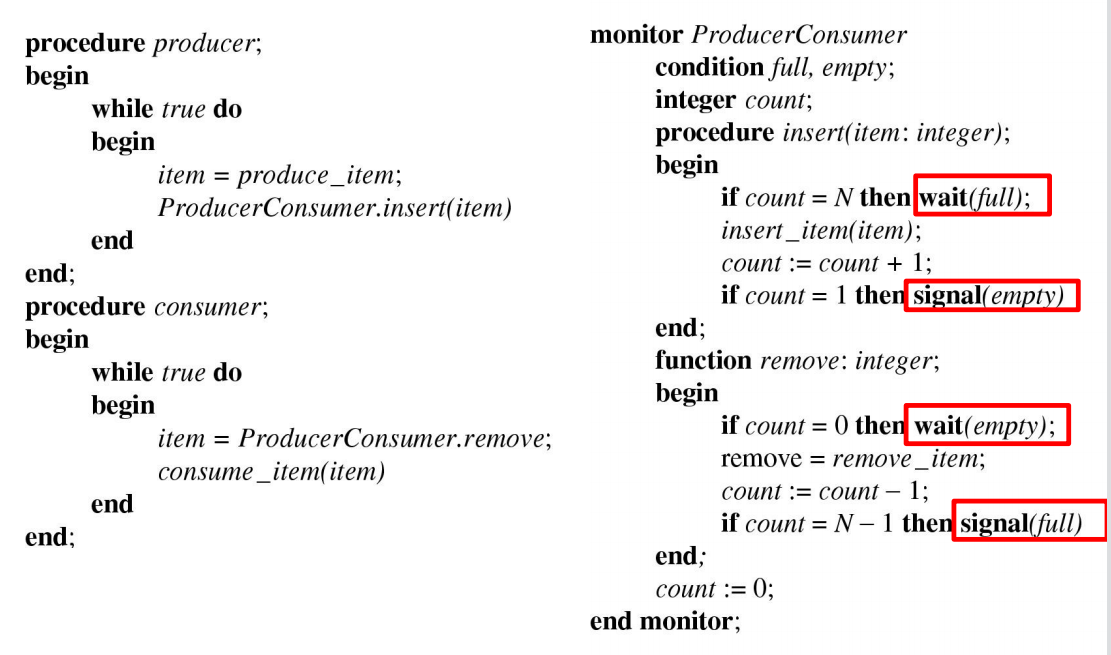
\includegraphics[width=\textwidth]{PCProblemMonitor.png}

\subsection{Atomic Locking – TSL Instruction}
\begin{itemize}
    \item Instruction format: TSL Register, Lock
    \item Lock \begin{itemize}
        \item Located in memory. 
        \item Has a value of 0 or 1
    \end{itemize}
    \item Register: One of CPU registers
    \item TSL does the following two operations {\bfseries atomically (as one step)} \begin{itemize}
        \item Register := Lock; // Copy the old value of Lock to Register
        \item Lock := 1; // Set the new value of Lock to 1
    \end{itemize}
    \item TSL is a basic primitive using which other more complex locking mechanisms can be implemented.
\end{itemize}
Implementation of Mutex Using TSL
\newline
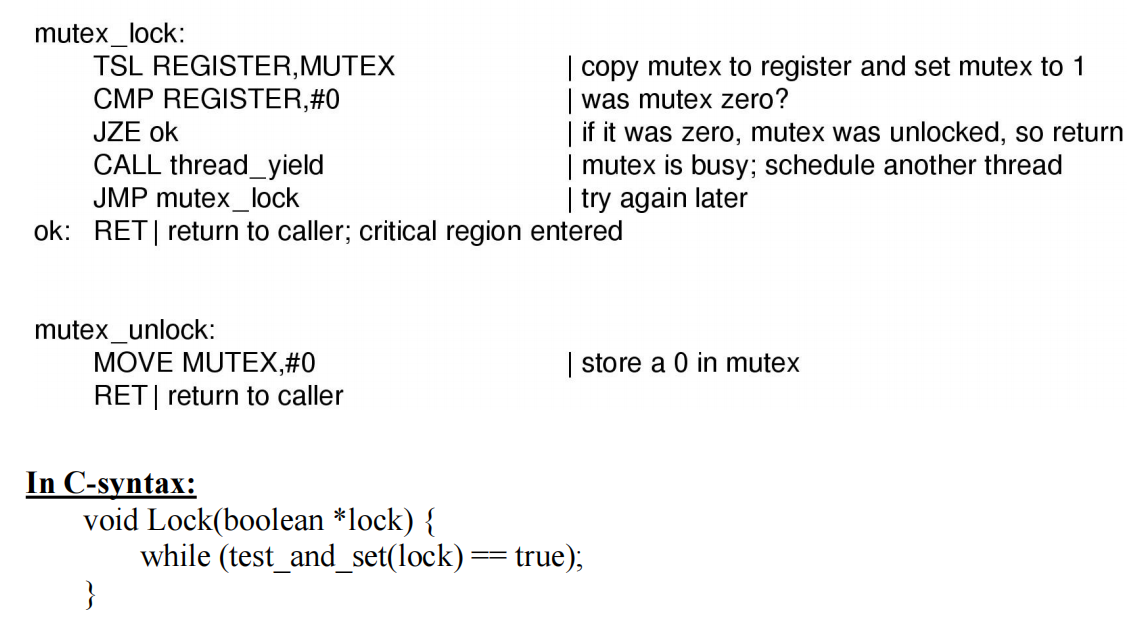
\includegraphics[width=\textwidth]{TSLImplementation.png}

\section{Kernel Modules}
\subsection{Definition}
\begin{itemize}
    \item Allow code to be added to the kernel, dynamically 
    \item Only those modules that are needed are loaded. Unload when no longer required - frees up memory and other resources 
    \item Reduces kernel size. 
    \item Enables independent development of drivers for different 
    devices
\end{itemize}
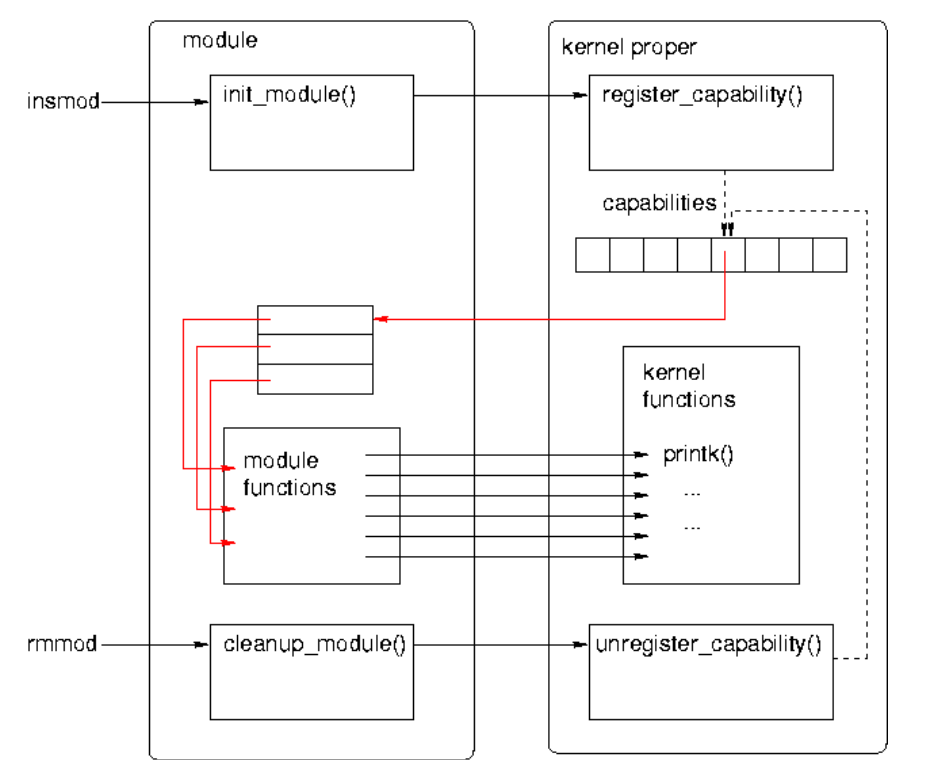
\includegraphics[width=\textwidth]{KernelWorking.png}
\subsection{Development}
\subsubsection{Hello World Example}
\begin{lstlisting}
    #include <linux/init.h> 
    #include <linux/module.h> 
    MODULE_LICENSE("DUAL BSD/GPL"); 
    // called when module is installed 
    int __init hello_init() 
    { 
     printk(KERN_ALERT "mymodule: Hello World!\n"); 
     return 0; 
    } 
    // called when module is removed 
    void __exit hello_exit() 
    { 
     printk(KERN_ALERT "mymodule: Goodbye, cruel world!!\n"); 
    } 
    module_init(hello_init); 
    module_exit(hello_exit);
\end{lstlisting}
\subsubsection{Compile}
\begin{itemize}
    \item Makefile \begin{itemize}
        \item \textcolor{blue}{obj-m := testmod.o}
        \item For multiple files: \textcolor{blue}{module-objs := file1.o file2.o}
    \end{itemize}
    \item Compiling: \$ make -C /lib/modules/\$(uname -r)/build M=`pwd` modules
\end{itemize}
\subsubsection{Module Utilities}
\begin{itemize}
    \item \textcolor{blue}{sudo insmod hello.ko} \begin{itemize}
        \item Inserts a module
        \item Internally, makes a call to sys\_init\_module
        \item Calls vmalloc() to allocate kernel memory
        \item Copies module binary to memory
        \item Resolves any kernel references (e.g. printk) via kernel symbol table
        \item Calls module’s initialization function
    \end{itemize}
    \item \textcolor{blue}{modprobe hello.ko}: Same as insmod, except that it also loads any other modules that hello.ko references
    \item \textcolor{blue}{sudo rmmod hello} \begin{itemize}
        \item Removes a module
        \item Fails if module is still in use
    \end{itemize}
    \item \textcolor{blue}{sudo lsmod} \begin{itemize}
        \item Tells what modules are currently loaded 
        \item Internally reads /proc/modules
    \end{itemize}
\end{itemize}
\subsubsection{Things to Remember}
\begin{itemize}
    \item Modules can call other kernel functions, such as printk, kmalloc, kfree, but only the functions that are EXPORTed by the kernel(using EXPORT(symbol\_name))
    \item Modules (or any kernel code for that matter) cannot call user-space library functions, such as  malloc, free, printf etc.
    \item Modules should not include standard header files, such as stdio.h, stdlib.h, etc.
    \item Segmentation fault may be harmless in user space, but a kernel fault can crash the entire system
    \item Version Dependency: Module should be recompiled for each version of kernel that it is linked to
\end{itemize}
\subsubsection{Concurrency Issues}
\begin{itemize}
    \item Many processes could try to access your module concurrently. So different parts of your module may be active at the same time
    \item Device interrupts can trigger Interrupt Service Routines (ISR), ISRs may access common data that your module uses as well
    \item Kernel timers can concurrently execute with your module and access common data
    \item You may have symmetric multi-processor (SMP) system, so multiple processors may be executing your module code simultaneously (not just concurrently).
    \item Therefore, your module code (and most kernel code, in general) should be re-enterant, Capable of correctly executing correctly in more than one context simultaneously
\end{itemize}
\subsubsection{Error Handling}
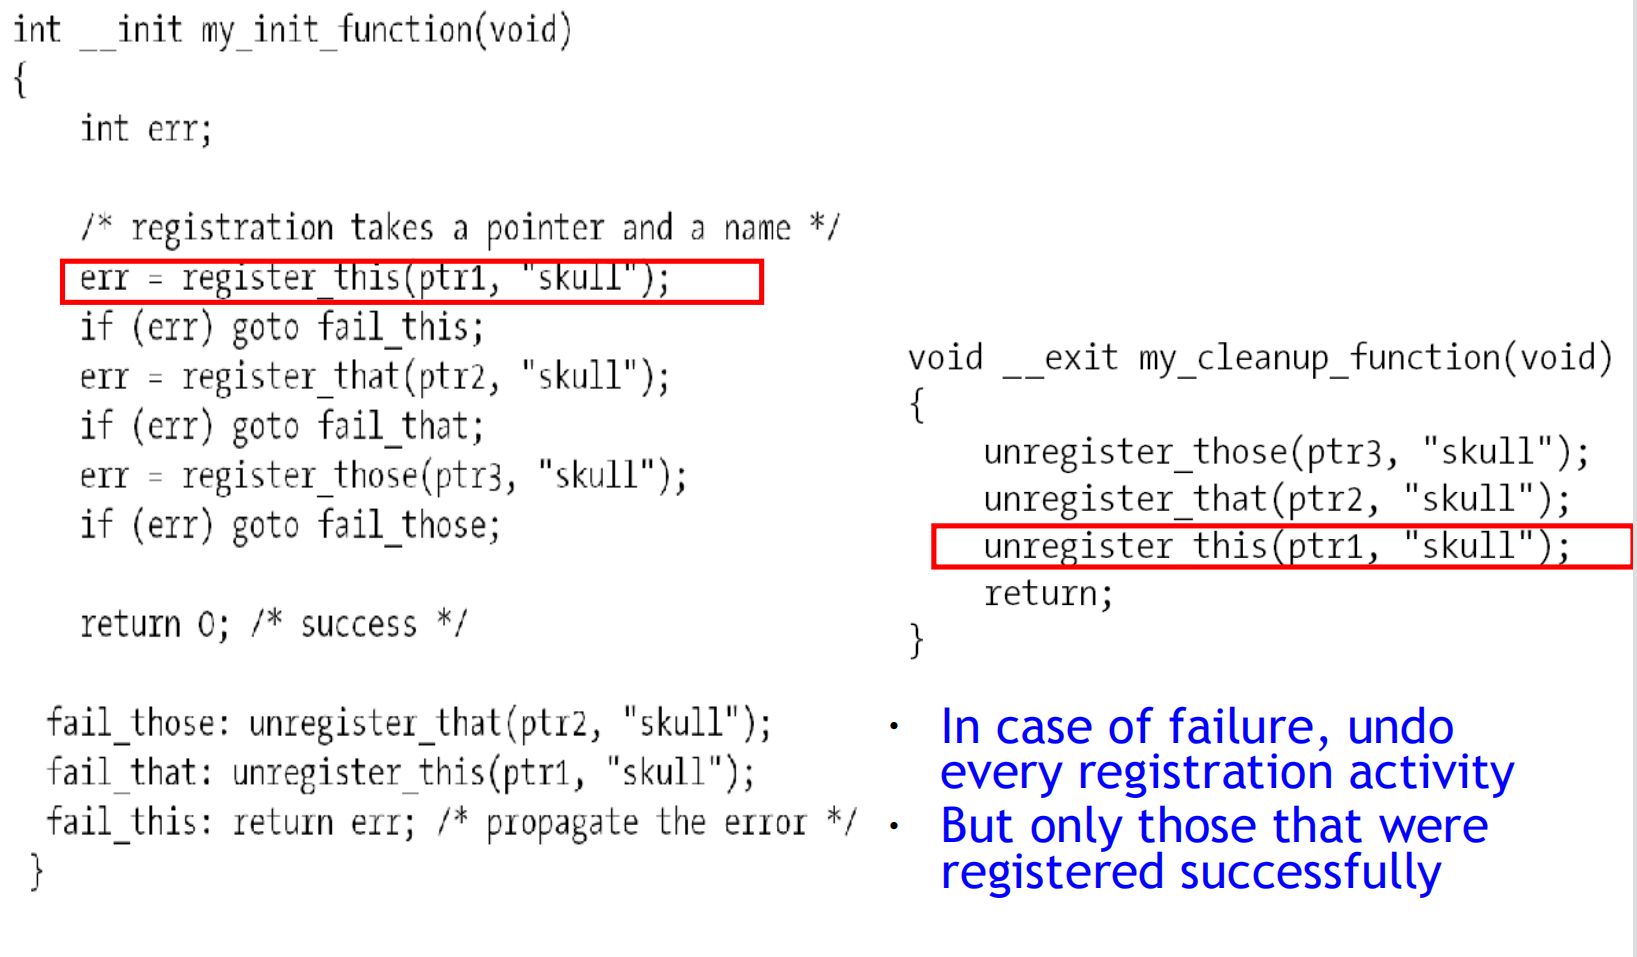
\includegraphics[width=\textwidth]{KernelErrorHandling.png}
\subsubsection{Module Parameters}
\begin{itemize}
    \item Command line: \textcolor{blue}{insmod hellon.ko howmany=10 whom="Class"}
    \item Module code has: \begin{lstlisting}
        static char *whom = "world";
        static int howmany = 1;
        module_param(howmany, int, S_IRUGO);
        module_param(whom, charp, S_IRUGO);
    \end{lstlisting}
\end{itemize}
\subsection{Character devices in Linux}
\subsubsection{Device Classification}
\begin{itemize}
    \item Character (char) devices \begin{itemize}
        \item byte-stream abstraction(keyboard, mouse)
    \end{itemize}
    \item Block devices \begin{itemize}
        \item reads/writes in fixed block granularity (hard disks, CD drives)
    \end{itemize}
    \item Network devices \begin{itemize}
        \item message abstraction, send/receive packets of varying sizes (network interface cards)
    \end{itemize}
    \item Others \begin{itemize}
        \item USB, SCSI, Firewire, I2O
        \item Can (mostly) be used to implement one or more of the above three classes
    \end{itemize}
\end{itemize}
\subsubsection{"Miscellaneous" Devices in Linux}
\begin{itemize}
    \item These are character devices used for simple device drivers. 
    \item All miscellaneous devices share a major number (10). 
    \item But each device gets its own minor number, requested at registration time
\end{itemize}
\subsubsection{Implementing a device driver for a miscellaneous device}
\begin{enumerate}
    \item  Declare a device struct \begin{lstlisting}
        static struct miscdevice my_misc_device = {
        .minor = MISC_DYNAMIC_MINOR,
        .name = "my device",
        .fops = &my_fops
    };
    \end{lstlisting}
    \item Declare the file operations struct \begin{lstlisting}
        static struct file_operations my_fops = {
            .owner = THIS_MODULE,
            .open = my_open,
            .release = my_close,
            .read = my_read,
            ...
            .llseek = noop_llseek
        };
        // The function pointers that are not initialized above will be assigned some sensible default value by the kernel.
    \end{lstlisting}
    \item register the device with kernel, usually in the module initialization code \begin{lstlisting}
        static int __init my_module_init()
        {
            ...
            misc_register(&my_misc_device);
            ...
        }
        // And don't forget to unregister the device when removing the module
        static void __exit my_exit(void)
        {
            misc_deregister(&my_misc_device);
            ...
        }
    \end{lstlisting}
    \item Implement the fops functions \begin{lstlisting}
        static ssize_t my_read(struct file *file, char __user * out, size_t size, loff_t * off)
        {
            ...
            sprintf(buf, "Hello World\n");
            copy_to_user(out, buf, strlen(buf)+1);
            ...
        }
    \end{lstlisting}
    \item Warning \begin{itemize}
        \item allocate memory for buf
        \item Check if "out" points to a valid user memory location using\ access\_OK()
        \item check for errors during copy\_to\_user()
    \end{itemize}
\end{enumerate}
\subsubsection{How do file ops work on character devices}
\begin{itemize}
    \item A file operation on a device file will be handled by the kernel module associated with the device
    \item Use "open()" system call to open "mydevice" file \begin{itemize}
        \item fd = open("/dev/mydevice", O\_RDWR); 
        \item opens /dev/mydevice device for read and write operation. 
        \item OS will call my\_open() file operation handler in the kernel module which is associated with the device. 
        \item misc\_register(\&my\_misc\_device) in my\_module\_init() registers the character device. It creates an entry in the "/dev" directory for "mydevice" file and informs the operating system what file-operations handler functions are available for this device.
    \end{itemize}
    \item Use "read()" system call to read from the "mydevice" file \begin{itemize}
        \item n = read( fd, buffer, size);
        \item finally calls the my\_read() function passed through the fops structure in your kernel module
    \end{itemize}
\end{itemize}
\subsubsection{Moving data in and out of the Kernel}
\begin{itemize}
    \item copy\_to\_user() \begin{itemize}
        \item unsigned long copy\_to\_user (void \_\_user * dst, const void * src, unsigned long n)
        \item Copies data from kernel space to user space
        \item Returns number of bytes that could not be copied. On success, this will be zero.
        \item Checks that dst is writable by calling access\_ok on dst with a type of VERIFY\_WRITE. If it returns non-zero, copy\_to\_user proceeds to copy
    \end{itemize}
    \item copy\_from\_user() \begin{itemize}
        \item unsigned long copy\_from\_user (void * dst, const void \_\_user * src, unsigned long n)
        \item Copies data from user space to kernel
        \item Returns number of bytes that could not be copied. On success, this will be zero
    \end{itemize}
\end{itemize}
\subsubsection{Memory allocation/deallocation in Kernel}
\begin{itemize}
    \item Memory Allocation: \begin{itemize}
        \item kmalloc(): Allocates physically contiguous memory: \begin{lstlisting}
            void * kmalloc(size_t size, int flags)
        \end{lstlisting}
        \item kzalloc(): Allocates memory and sets it to zero
        \item vmalloc(): Allocates memory that is virtually contiguous and not necessarily physically contiguous.
    \end{itemize}
    \item Memory Deallocation: kfree()
\end{itemize}

\section{System Calls}
\subsection{Definition}
\begin{itemize}
    \item Interface to allow User-level processes to safely invoke OS routines for privileged operations
    \item Safely transfer control from lower privilege level (user mode) to higher privilege level (supervisor mode), and back
\end{itemize}
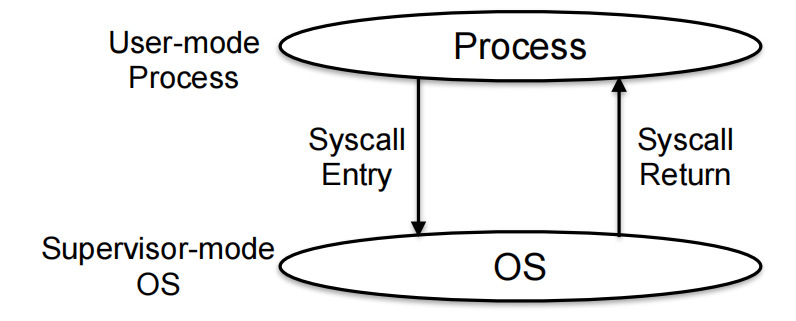
\includegraphics[width=\textwidth]{SystemCalls.png}
\subsubsection{System Call table}
\begin{itemize}
    \item \textcolor{blue}{Protected entry points} into the kernel for each system call: We don’t want application to randomly jump into any part of the OS code
    \item Syscall table is usually implemented as an array of function pointers, where each function implements one system call
    \item Syscall table is indexed via system call number
\end{itemize}
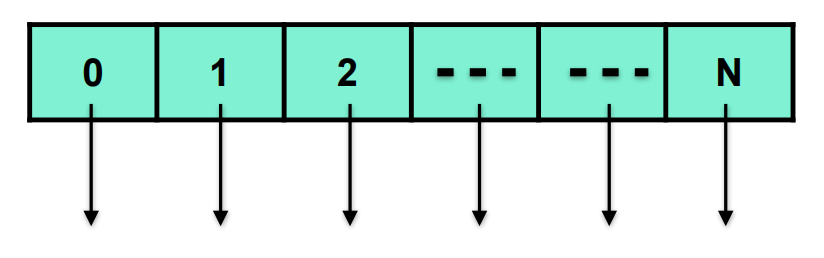
\includegraphics[width=0.8\textwidth]{SystemCallTable.png}
\subsubsection{System Call Invocation}
\begin{enumerate}
    \item System calls is invoked via a special CPU instruction: The system call number and arguments passed via CPU registers and optionally stack
    \item CPU saves process execution state
    \item CPU switches to higher privilege level: jumps to an entry point in OS code
    \item OS indexes the system call table using the system call number
    \item OS invokes the system call via a function pointer in the system call table \begin{itemize}
        \item For performance reasons, the system call usually executes in the execution context of the calling process, but in privileged mode
        \item Some OS may execute the system call in a separate execution context for better security
    \end{itemize}
    \item If the syscall involves blokcing I/O, the calling process may block while the I/O completes
    \item When syscall completes, the calling process is moved to ready state
    \item The saved process state is restored
    \item Processor switches back to lower privilege level using SYSEXIT/iret instructions
    \item Process returns from the system call and continues.
\end{enumerate}
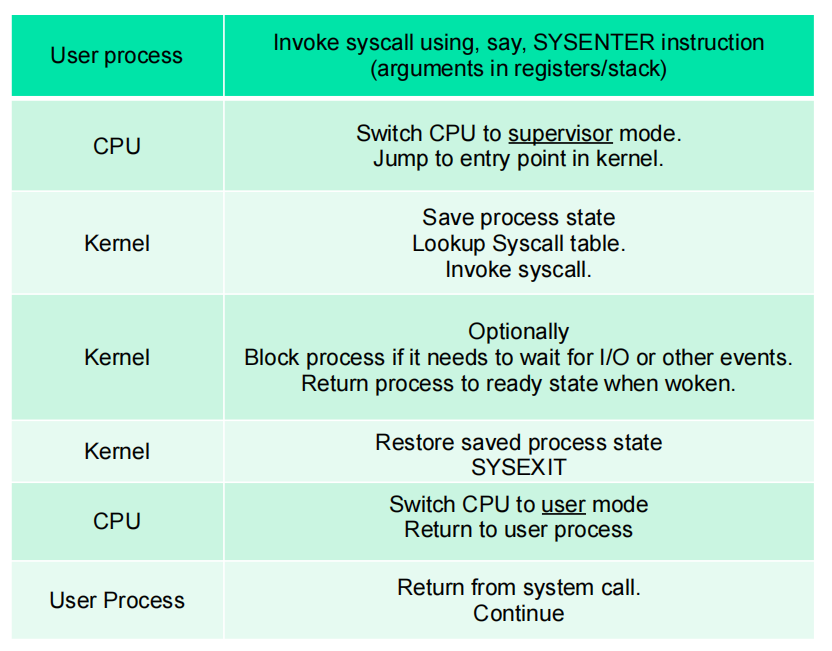
\includegraphics[width=\textwidth]{SystemCallExecution.png}
\subsection{Syscall Usage}
\begin{itemize}
    \item To make it easier to invoke system calls, OS writers normally provide a library that sits between programs and system call interface: Libc, glibc, etc 
    \item This library provides wrapper routines
    \item Wrappers hide the low-level details of \begin{itemize}
        \item Preparing arguments
        \item Passing arguments to kernel 
        \item Switching to supervisor mode
        \item Fetching and returning results to application
    \end{itemize}
    \item Helps to reduce OS dependency and increase portability of programs
\end{itemize}
\subsection{Implementing}
\subsubsection{Steps in Writing a System Call}
\begin{enumerate}
    \item Create an entry for the system call in the kernel’s \textcolor{blue}{syscall\_table}: User processes trapping to the kernel (through SYS\_ENTER or int 0x80) find the syscall function by indexing into this table
    \item Write the system call code as a kernel function \begin{itemize}
        \item Be careful when reading/writing to user-space
        \item Use copy\_to\_user() or copy\_from\_user() routines. These perform sanity checks.
    \end{itemize}
    \item Implement a user-level wrapper to invoke your system call: Hides the complexity of making a system call from user applications.
\end{enumerate}
\subsubsection{Code}
\begin{enumerate}
    \item Create a sys\_call\_table entry (for 64-bit x86 machines):Syscall table initialized in arch/x86/entry/syscall\_64.c \begin{lstlisting}
        # 
        # 64-bit system call numbers and entry vectors 
        # 
        # The format is: 
        # <number> <abi> <name> <entry point> 
        # 
        # The abi is "common", "64" or "x32" for this file. 
        ... 
        309 common getcpu sys_getcpu 
        310 64 process_vm_readv sys_process_vm_readv 
        311 64 process_vm_writev sys_process_vm_writev 
        312 common kcmp sys_kcmp 
        313 common foo sys_foo
    \end{lstlisting}
    \item Write the system call handler \begin{itemize}
        \item System call with no arguments and integer return value \begin{lstlisting}
            SYSCALL_DEFINE0(foo){ 
                printk (KERN ALERT "sys_foo: pid is %d\n", current->pid); 
                return current->pid; 
            }
        \end{lstlisting}
        \item Syscall with one primitive argument \begin{lstlisting}
            SYSCALL_DEFINE1(foo, int, arg){
                printk (KERN ALERT "sys_foo: Argument is %d\n", arg); 
                return arg;
            }
        \end{lstlisting}
        \item To see system log: \begin{itemize}
            \item dmesg
            \item less /var/log/kern.log
        \end{itemize}
        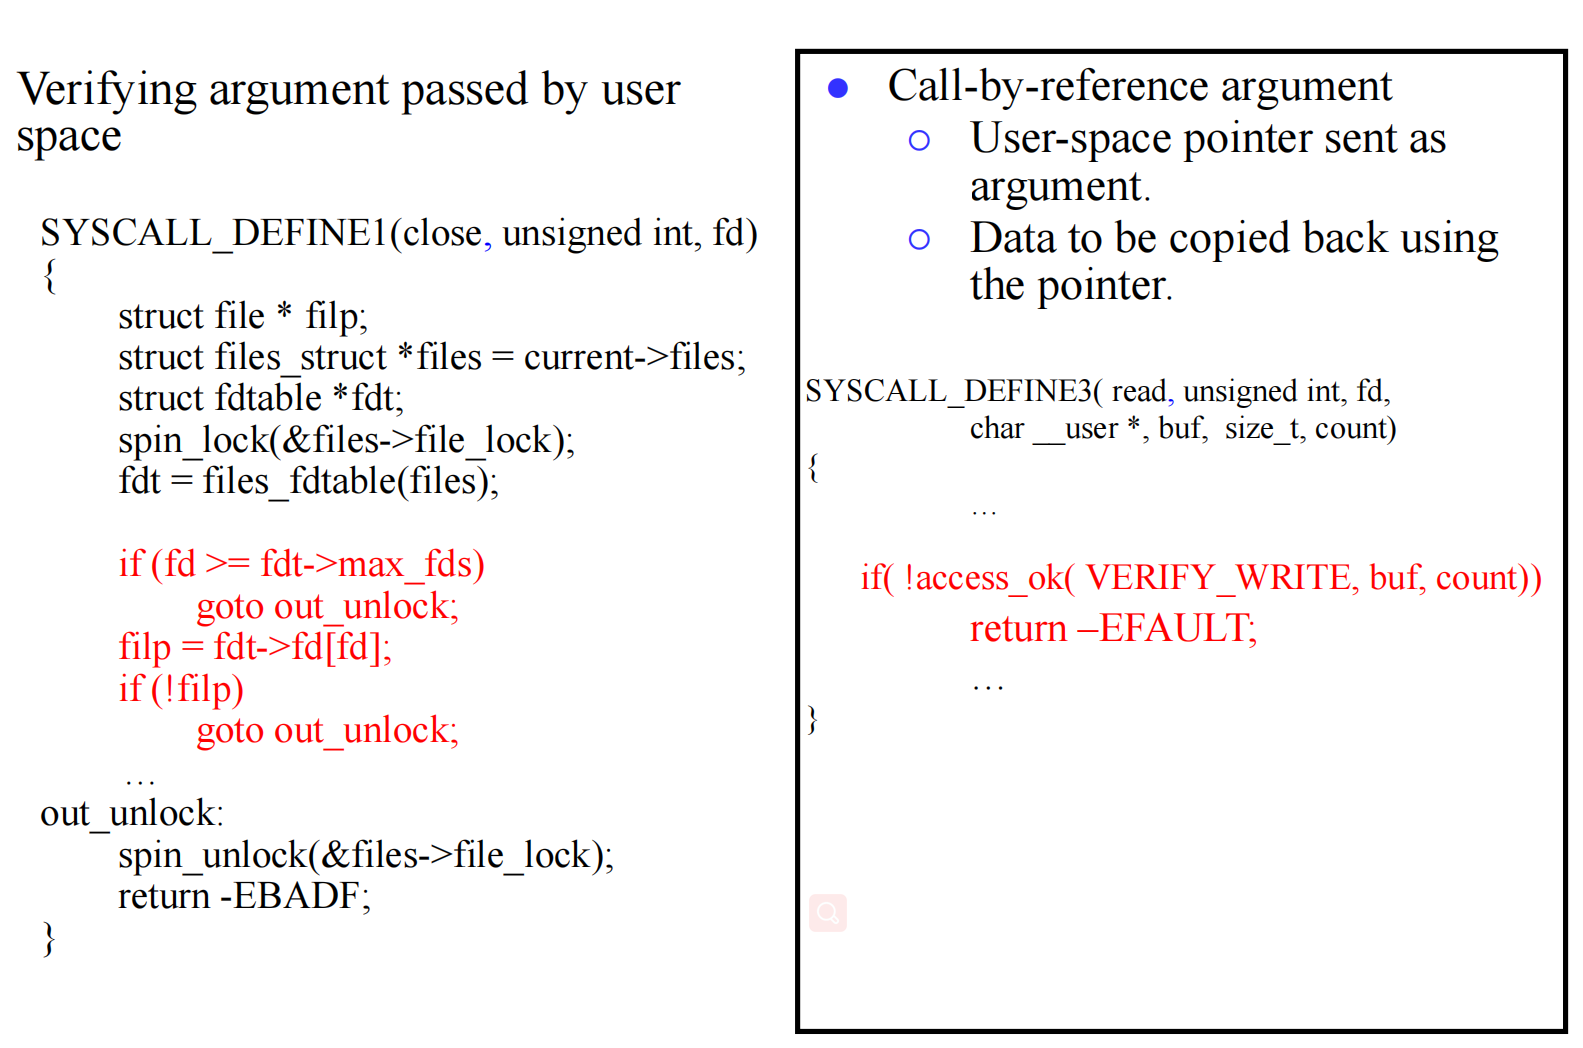
\includegraphics[width=0.8\textwidth]{SystemCallHandler.png}
    \end{itemize}
    \item Invoke syscall handler from user space \begin{itemize}
        \item Use the syscall(...) library function.
        \item For instance, for a no-argument system call named foo(), you'll call \begin{lstlisting}
            ret = syscall(__NR_sys_foo);
        \end{lstlisting}
        \item For a 1 argument system call named foo(arg), you call \begin{lstlisting}
            ret = syscall(__NR_sys_foo, arg);
        \end{lstlisting}
        \item and so on for 2, 3, 4 arguments etc.
    \end{itemize}
\end{enumerate}

\section{Memory Management}
Ideally programmers want memory that is
\begin{itemize}
    \item Large
    \item Fast
    \item Persistent
\end{itemize}

\subsection{Memory Hierarchy}
\begin{itemize}
    \item Registers \& Cache: small amount of fast, expensive, volatile memory
    \item Main memory: some medium-speed, medium price, volatile/persistent memory, DRAM
    \item Disk \& Tape: Lots of slow, cheap, persistent, storage
\end{itemize}
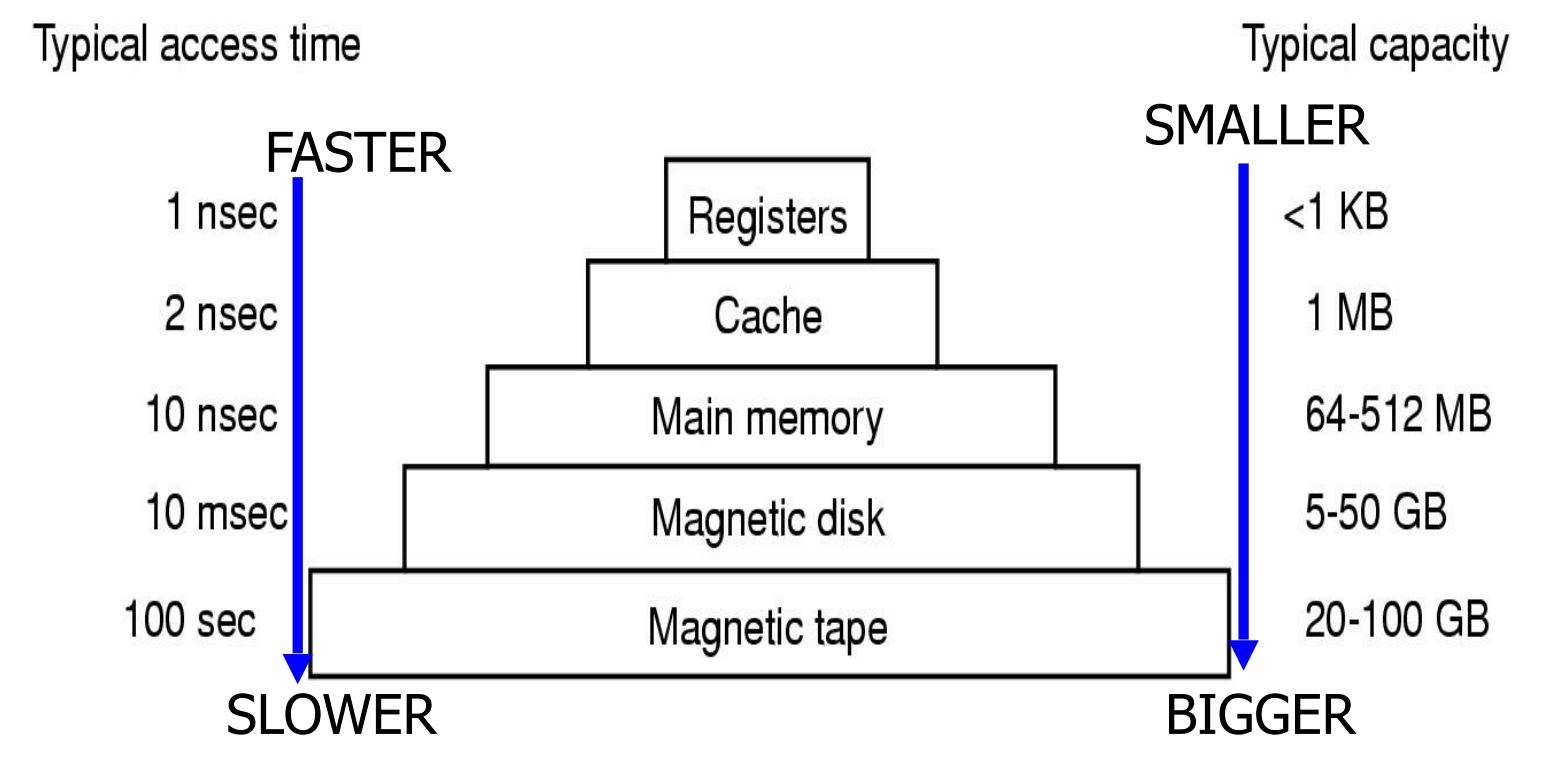
\includegraphics[width=\textwidth]{MemoryHierarchy.png}

\subsection{Relocation and Protection}
\begin{itemize}
    \item Problem: A programmer doesn’t know where a program will be loaded in memory \begin{itemize}
        \item address locations of variables and code routines cannot be absolute
        \item must keep a program out of other processes’ partitions
    \end{itemize}
    \item Solution: Use base and limit values
    \item Relocation \begin{itemize}
        \item Address locations in a program are relative
        \item They are added to a base value to map to physical addresses
    \end{itemize}
    \item Protection: Access to address locations larger than limit value results in an error
\end{itemize}
\subsection{Swapping}
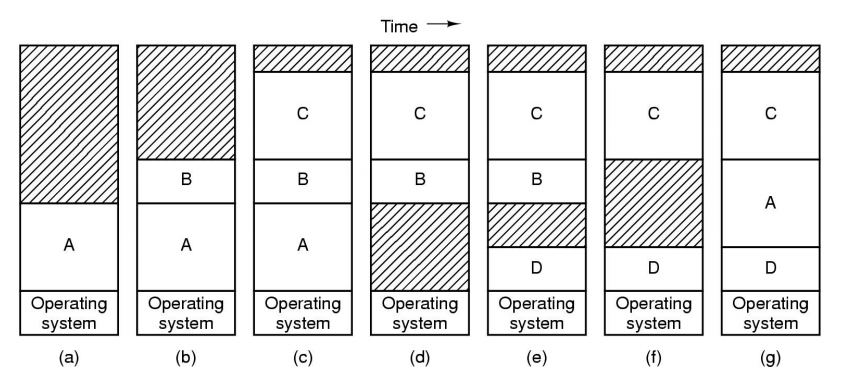
\includegraphics[width=\textwidth]{Swapping.png}
\begin{itemize}
    \item Physical memory may not be enough to accommodate the needs of all processes
    \item Memory allocation changes as \begin{itemize}
        \item processes come into memory
        \item leave memory and are swapped out to disk
        \item Re-enter memory by getting swapped-in from disk
    \end{itemize}
    \item Shaded regions are unused memory
\end{itemize}
\subsection{Paging}
\begin{itemize}
    \item Swapping the memory of an entire process is useful when the sum of memory needed by all processes is greater than the total RAM available in the system. 
    \item But sometimes, a single process might require more memory than the total RAM in the system. 
    \item In such cases swapping an entire process is not enough. 
    \item Rather, we need to break up the memory space of a process into smaller equal-sized pieces, called PAGES. 
    \item OS then decides which pages stay in memory and which get moved to disk.
    \item \textcolor{red}{Virtual memory}: means that each process gets an illusion that it has more memory than the physical RAM in the system
\end{itemize}
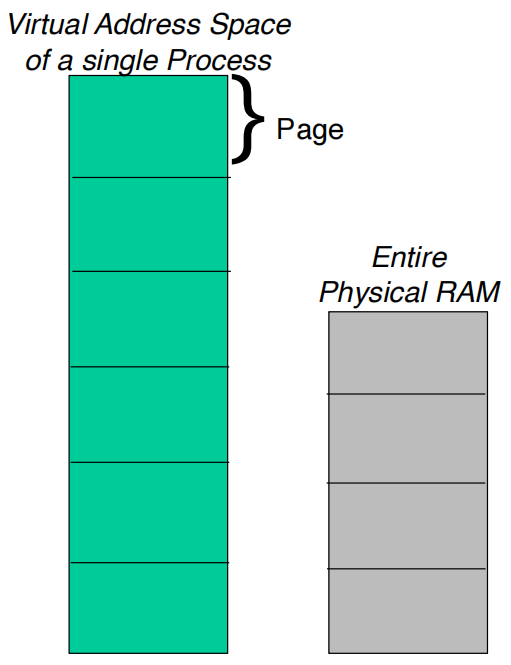
\includegraphics[width=0.6\textwidth]{Paging.png}
\subsection{Memory Management Unit (MMU)}
\begin{itemize}
    \item MMU is a hardware module that accompanies the CPU
    \item It translates the Virtual Address used by executing instructions to Physical Addresses in the main memory
    \item It need to be very quick so it stands along with CPU
    \item Steps \begin{enumerate}
        \item CPU tells MMU the virtual address P it needs
        \item MMU translante P into P* which is the physical address 
        \item P* is sent through Bus to the memory controller
        \item memorry controller get the P* data and send it back by Bus
    \end{enumerate}
\end{itemize}
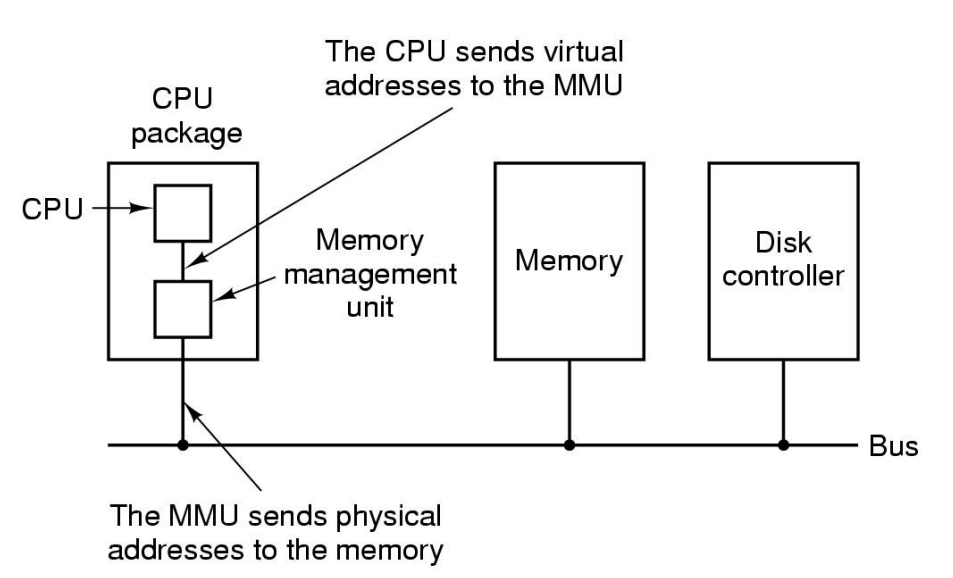
\includegraphics[width=\textwidth]{MemoryManagementUnit.png}
\subsection{Size of address space (in bytes) as a function of address size (in bits)}
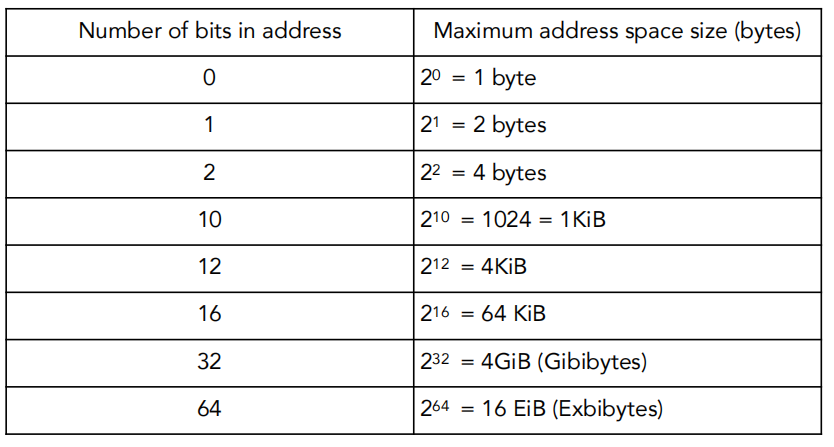
\includegraphics[width=\textwidth]{AddressSpaceSize.png}
\subsection{PageTable}
\begin{itemize}
    \item An array that stores the mapping from virtual page numbers to physical numbers
    \item The OS maintains \begin{itemize}
        \item \textcolor{blue}{One page table per userspace process}
        \item And usually another page table for kernel memory
    \end{itemize}
\end{itemize}
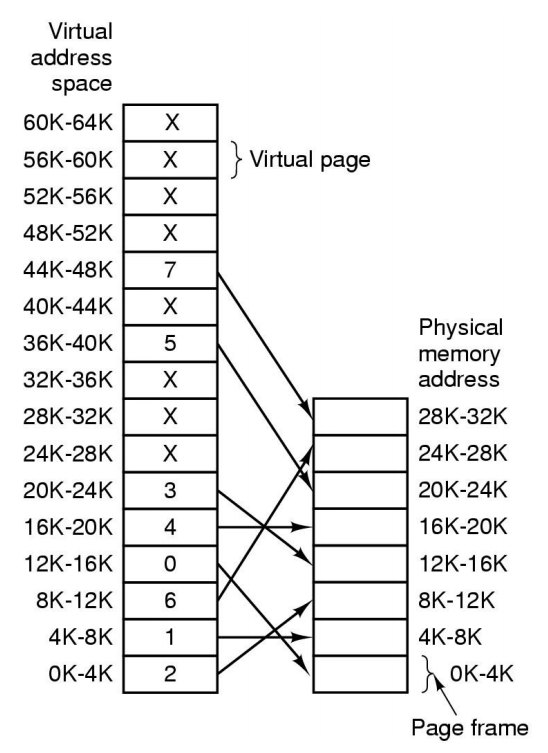
\includegraphics[width=0.6\textwidth]{PageTable.png}
\subsection{Traslate Virtual address (VA) to physical address (PA)}
\begin{itemize}
    \item Byte Address = Page Number x Page Size + Byte Offset in the page
    \item VA = VPN x Page Size + Byte Offset
    \item PA = PPN x Page Size + Byte Offset
\end{itemize}
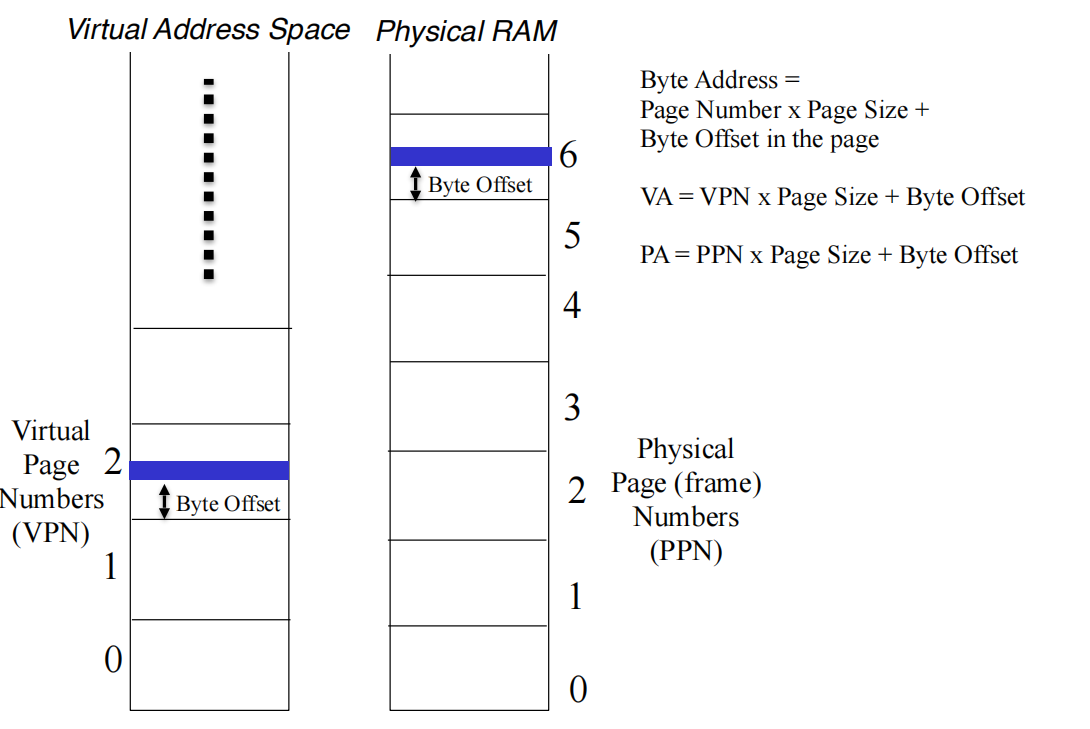
\includegraphics[width=\textwidth]{VAtoPA.png}
\subsubsection{Virtual Address Translation For Small Address Space}
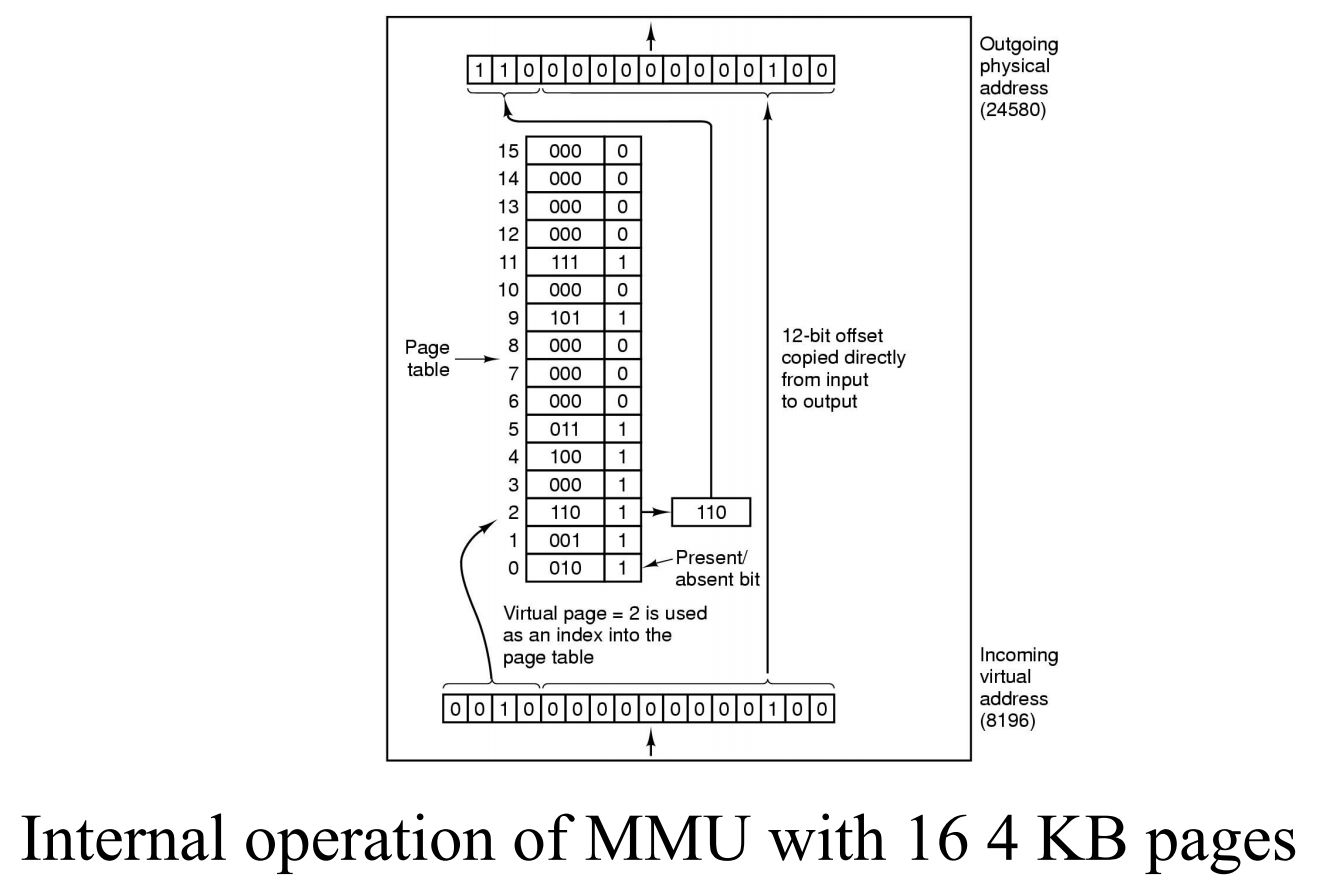
\includegraphics[width=\textwidth]{VATranslationExample.png}
\begin{itemize}
    \item The first 12 bits: byte Offset
    \item The last 4 bits: virtual page number
    \item Page fault: the absent bit in page table is 0 \begin{itemize}
        \item OS would fix the entry
        \item Rerun the instruction
    \end{itemize}
    \item Each process has its own page table, it used to need to be load in the MMU, but as the bit of computer grows, the MMU need to be got out to the DRAM. \begin{itemize}
        \item page table's entry number becomes larger and larger: a 32-bit computer has over 1 million entries for each process's page table, which significantly decreases the speed of switching context.
        \item the storage cost is too expensive
    \end{itemize}
    \item so MMU keeps a pointer(mostly a register) to the DRAM which is the base of physical memory address
    \item Problem: what if the contiguous memory is hard to find? Different layer of page table
    \item Problem: what if the translation is inefficient? Store a small page table in MMU in the cache, it's called TLB. If we can find the physical memory in TLB, it's a hit. Otherwise it's a miss, go to DRAM.
\end{itemize}
\subsubsection{Virtual Address Translation For Large Address Space}
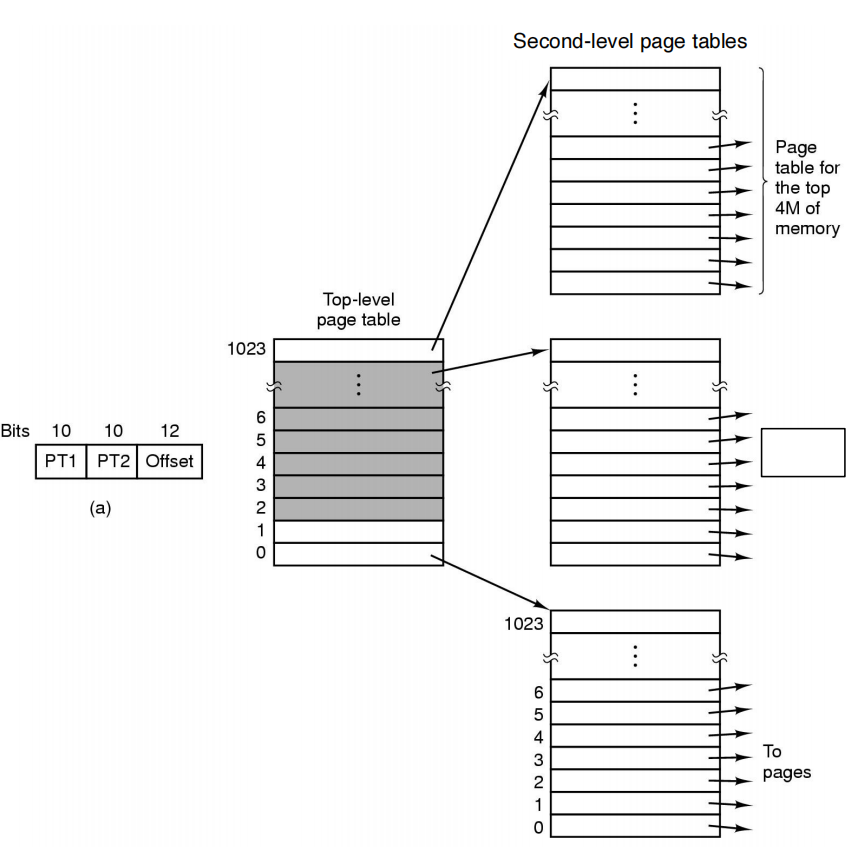
\includegraphics[width=\textwidth]{VATranslationExampleBig.png}
\begin{itemize}
    \item 32 bit address with 2 page table fields
    \item Two-level page tables
    \item PT too Big for MMU: Keep it in main memory
    \item But how does MMU know where to find PT? Registers (CR2 on Intel)
\end{itemize}
\subsection{Typical Page Table Entry (PTE)}
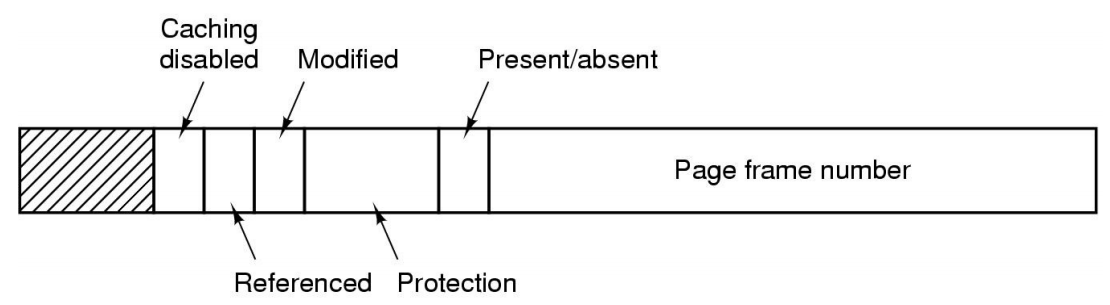
\includegraphics[width=\textwidth]{PTE.png}
\begin{itemize}
    \item Page Frame number = physical page number for the virtual page represented by the PTE
    \item Referenced bit: Whether the page was accessed since last time the bit was reset.
    \item Modified bit: Also called "Dirty" bit. Whether the page was written to, since the last time the bit was reset.
    \item Protection bits: Whether the page is readable? writeable? executable? contains higher privilege code/data?
    \item Present/Absent bit: Whether the PTE contains a valid page frame number. Used for marking swapped/unallocated pages
    \item Cashing disabled bit: point to some I/O devices(memory map I/O) rather than memory
\end{itemize}
\subsection{TLBs – Translation Lookaside Buffers}
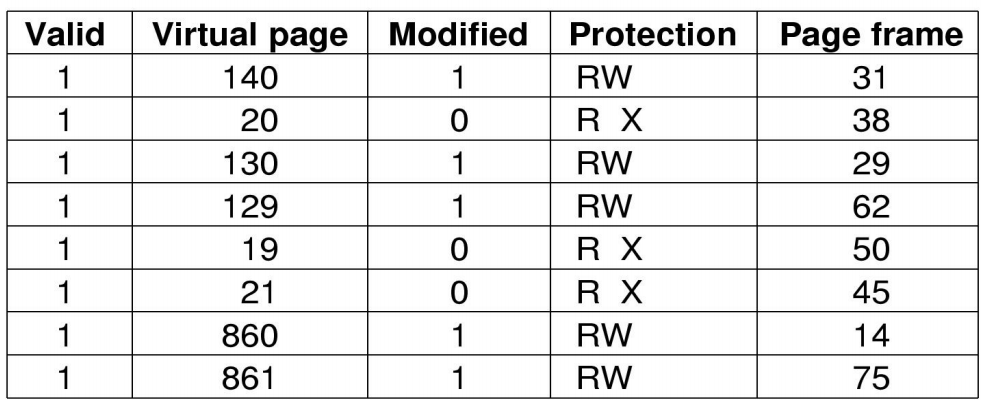
\includegraphics[width=\textwidth]{TLB.png}
\begin{itemize}
    \item TLB is a small cache that speeds up the translation of virtual addresses to physical addresses.
    \item TLB is part of the MMU hardware (comes with CPU)
    \item TLB is made of fully associative cache, which could compare all the entries at the same time.
    \item It is not a Data Cache or Instruction Cache. Those are separate.
    \item TLB simply caches translations from virtual page number to physical page number so that the MMU don’t have to access page-table in memory too often.
    \item On older x86 processors, TLB had to be “flushed” upon every context switch because there is no field in TLB to identify the process context. Tagged TLB can reduce this overhead, it use ASID to remember its owner process.
    \item Spatial Locality: if the process is accessing i byte, it's very likely it will access nearby bytes.
    \item Temporal Locality: if the process is accessing i byte, it's very likely it will keep accessing i byte in the future
    \item If CPU do a context switch, all the valid bits will be set to 0, and the new process needs to take some time to get in a new page table. There will be misses at first, but as PLB warms up, it will be hit eventually.
\end{itemize}
\subsection{Impact of Page Size on Page tables}
\subsubsection{Small Page Size}
\begin{itemize}
    \item Advantages \begin{itemize}
        \item less internal fragmentation(space wasted)
        \item page-in/page-out less expensive
    \end{itemize}
    \item Disadvantages \begin{itemize}
        \item process that needs more pages has larger page table
        \item Smaller “TLB Coverage” (next slide)
    \end{itemize}
\end{itemize}


\end{document}